\documentclass[
  a4paper,BCOR10mm,oneside,
  bibtotoc,idxtotoc,
  headsepline,footsepline,% also activate headinclude and footinclude
  fleqn,openbib
]{scrbook}
\usepackage[automark]{scrpage2}
\usepackage[ngerman,english]{babel}% default language as last entry
\usepackage[utf8]{inputenc}
\usepackage{amsmath} 
\usepackage{amsfonts}
\usepackage{amssymb}
\usepackage{graphicx}
\usepackage{lastpage}% to get last page use \pageref{LastPage}
\usepackage[refpage,intoc]{nomencl}% for nomenlature Abkuerzungsverzeichnis
\usepackage{listings}
\usepackage{color}

\definecolor{mygreen}{rgb}{0,0.6,0}
\definecolor{mygray}{rgb}{0.5,0.5,0.5}
\definecolor{mymauve}{rgb}{0.58,0,0.82}

\lstset{ %
  backgroundcolor=\color{white},   % choose the background color; you must add \usepackage{color} or \usepackage{xcolor}
  basicstyle=\footnotesize,        % the size of the fonts that are used for the code
  breakatwhitespace=false,         % sets if automatic breaks should only happen at whitespace
  breaklines=true,                 % sets automatic line breaking
  captionpos=b,                    % sets the caption-position to bottom
  commentstyle=\color{mygreen},    % comment style
  deletekeywords={...},            % if you want to delete keywords from the given language
  escapeinside={\%*}{*)},          % if you want to add LaTeX within your code
  extendedchars=true,              % lets you use non-ASCII characters; for 8-bits encodings only, does not work with UTF-8
  frame=single,	                   % adds a frame around the code
  keepspaces=true,                 % keeps spaces in text, useful for keeping indentation of code (possibly needs columns=flexible)
  keywordstyle=\color{blue},       % keyword style
  language=Octave,                 % the language of the code
  otherkeywords={*,...},           % if you want to add more keywords to the set
  numbers=left,                    % where to put the line-numbers; possible values are (none, left, right)
  numbersep=5pt,                   % how far the line-numbers are from the code
  numberstyle=\tiny\color{mygray}, % the style that is used for the line-numbers
  rulecolor=\color{black},         % if not set, the frame-color may be changed on line-breaks within not-black text (e.g. comments (green here))
  showspaces=false,                % show spaces everywhere adding particular underscores; it overrides 'showstringspaces'
  showstringspaces=false,          % underline spaces within strings only
  showtabs=false,                  % show tabs within strings adding particular underscores
  stepnumber=2,                    % the step between two line-numbers. If it's 1, each line will be numbered
  stringstyle=\color{mymauve},     % string literal style
  tabsize=2,	                   % sets default tabsize to 2 spaces
  title=\lstname                   % show the filename of files included with \lstinputlisting; also try caption instead of title
\makenomenclature
}

% define header and footer
\pagestyle{scrheadings}
\clearscrheadfoot % clear header and footer
\automark[section]{chapter}% !!! Wouldn't do that at oneside documents!!!
\ihead[]{\leftmark}% header left part
\ohead[]{\rightmark}% header right part
\ifoot{Name}% footer left part
\cfoot{Thema}% footer middle part
\makeatletter
% use different foot at front and main matter
\g@addto@macro{\mainmatter}{%
  \ofoot[{\usekomafont{pagenumber}Page \pagemark\ of \pageref{LastPage}}]
    {\usekomafont{pagenumber}Page \pagemark\ of 
      \pageref{LastPage}}% footer right part
}
\g@addto@macro{\frontmatter}{%
  \ofoot[\pagemark]{\pagemark}%
}
\makeatother


\begin{document}
\frontmatter% title pages are not numbered but counted!
\begin{titlepage}
  \raggedright% Use a different title style
  \null% page started
  \thispagestyle{empty}
  \selectlanguage{english}
  \vspace{4\baselineskip}
  \begin{tabular}{|ll@{}}
    & \\[\baselineskip]
    & \large Midtherm Report\\
    & \large Jan Grzegorzewski \\[\baselineskip]
    & \huge\textbf{Reaction-diffusion dynamics} \\
    & \huge\textbf{with fractional Brownian motion}\\[\baselineskip]
    & \large Summer term: 2016\\[2\baselineskip]
  \end{tabular}
\end{titlepage}

\tableofcontents
\listoffigures
\listoftables

\mainmatter
\selectlanguage{ngerman}
\selectlanguage{english}
\printnomenclature
\clearpage
\chapter{Introduction}

\chapter{Theory}
\section{Brownian Motion}
Gebrochene Brownische Bewegung ist eine Verallgemeinerung der Brownischen Bewegung. Sie kann benutzt werden bei der Simulation von Anomaler Diffusion.\newline \newline
Theorie von Felix, bisschen von Christoph und die Motivation könnte sein, dass man zwar anomale Diffusion simuliert werden kann wenn man alle Teilchen berücksichtigt. Mit diesem Ansatz könnte man konkret den Einfluss von Gebrochen-rationale Brownische Bewegung auf Reaktionen test.zb.als Vergleich zu normaler Brownian motion und Brownian Motion an sich ist auch schon eine Vereinfachung, welche eine zufällige Gaußzahl annimmt. Das heißt sämtliche Stöße des Teilchens mit anderen Teilchen innerhalb eines Zeitinvervalls werden schon zu diesem Wert verallgemeinert. Als Unterschied zu tatsächlichen Simulation von allen Stößen (MD-Simulation).
Die Motivation ist einen performanten Integrator für gebrochen-rationale Brownische Bewegung zu entwickeln. Die Anomale Diffusion, welche besonders in biologischen Systemen zu beobachten ist, wird durch Interaktion der Teilchen mit ihrer Umgebung verursacht. Für den im Verlauf verwendeten Integrator muss davon ausgegangen werden, dass keine weiteren Interaktion (Potentiale) auftreten. Da zur Erstellung der Trajektorie ihre sämtlichen Inkremente im voraus durch gewöhnliche Brownische Bewegung erstellt werden müssen. Der Vorteil von der Methode ist ihre Performance.  
Der hier verwendete Algorithmus leitet sich vom Davies-Haste Algorithmus \cite{Craigmile2003} ab.
Dabei werden anfänglich alle Inkremente (Geschwindigkeiten) für gewöhnliches Braunische Bewegung erzeugt $\eta_{Br}(t)= v(t)$. Für die Entfernung eines Teilchens zu seinem Ursprung gilt  $\Delta R(t)_{Br} = R(t)- R(0)= \int^t_{0}dt' v(t')$. Es ergibt sich für die Mittlere Quadratische Quadratische Verschiebung: \newline $\delta r^{2}_{norm}(t)= < \Delta R(t)_{Br}>=2dDt$ mit $d =\text{Anzahl der Dimension}$, $D = \text{Diffusionskonstante}$ und $t=$ Zeit. Da gewöhnliche Brownische Bewegung einer Gaußverteilung folgt und ein Markowischer Prozess ist,lässt sich für den Propagator  folgende Gleichung aufstellen:
\begin{equation}
 P(r,t)=[2 \pi \delta r^{2}_{norm}(t)/d]^{-\frac{d}{2}} e^{ \frac{-r^2 d}{2 \delta r^{2}_{norm}(t) }}
\end{equation}
\section{Fractional Brownian Motion}
Als Ausgangspunkt wird weiterhin die Differentialgleichung $\partial \boldsymbol{R}(t) = \boldsymbol{\eta}(t)$ betrachtet. $\eta_i(t)$ ist in dem Fall aber nicht mehr delta korreliert in der Zeit, wie für einfache Brownische Bewegung. Für Gebrochen-rationale Brownische Bewegung wird eine dauerhaftes Korrelation angenommen, sodass die Mittlere Quadratische Verschiebung nicht mit der für Brownische Bewegung übereinstimmt, aber stattdessen eine exponentielle Abhängigkeit zur Zeit aufweist $\delta r^{2}_{fBr}(t)= < \Delta R(t)_{fBr}>=2dK_{\alpha}t^{\alpha}$. 
%Für die Mittlere Quadratische Verschiebung gilt allgemein $\delta r^{2}_{fBr}(t) = \int^t_{0}dt' v(t')$ ...
Die Geschwindigkeitsautokorrelationsfunktion für Gebrochen-rationale Brownische Bewegung kann wie folgt definiert werden:
\begin{equation}
Z(\omega)= K_{\alpha} \Gamma(1+\alpha)(i z)^{1-\alpha} \text{   für} 
\end{equation}
\begin{itemize}
 \item $K_{\alpha} =$ generalisierter Diffusions-Koeffizient 
 \item $\omega = $ Frequenz 
\end{itemize}
\cite{Hofling2013}
\section{Algorythm}
Für den im Verlauf verwendeten Integrator muss davon ausgegangen werden, dass keine weiteren Interaktion (Potentiale) auftreten. Da zur Erstellung der Trajektorie ihre sämtlichen Inkremente im voraus durch gewöhnliche Brownische Bewegung erstellt werden müssen. Der Vorteil von der Methode ist ihre Performance. Der hier verwendete Algorithmus leitet sich vom Davies-Haste Algorithmus \cite{Craigmile2003} ab. Die theoretischen Überlegung aus dem Theorieteil müssen für den Algorithmus in eine diskrete Form gebracht werden. \\Das Inkrement ist:
\begin{align}
\boldsymbol{\eta} (t) \longrightarrow \boldsymbol{\eta}_j  \text{  mit  } j=(0,1,2,...,n)  \text{  und  } n= \text{ Schrittanzahl}
\end{align}
Die dickgeschriebenen Inkremente $\boldsymbol{\eta}_j$ sind als Vektoren zu verstehen. Die Schreibweise wird im Verlauf so belassen.
Es ergibt sich für die Länge der Trajektorie:
\begin{align}
 \Delta \boldsymbol{R}_n =  \sum_{j=0}^n \boldsymbol{\eta}_j  \Delta t \label{eq:diskretdeltar}
\end{align}
 Der Algorithmus hat die Motivation die Inkremente $ \boldsymbol{\eta}_j$so zu generieren, dass sie die Eigenschaften der Gebrochen-rationale Brownische Bewegung wiederspiegeln und sie insbesondere dem potentiellen Abklingen der Mittleren Quadratischen Verschiebung folgen.
\begin{align}
< \Delta \boldsymbol{R}_{fbr}>=2dK_{\alpha}t^{\alpha}
\end{align}
Der verwendete Algorithmus geht wie folgt:
 
\begin{enumerate}
 \item Es werden $2 n$ unabhängige Normalverteilte, mit dem Mittelwert $<\boldsymbol{n_j}>=0$ und der Standartabweichung $\delta \boldsymbol{n_j} = \sqrt{\Delta t}$, Zufallszahlen erstellt: 
 \begin{align}
  \boldsymbol{\eta_j}=(\boldsymbol{\eta_0},\boldsymbol{\eta_1},\boldsymbol{\eta_2},...,\boldsymbol{\eta_{2n}})= \boldsymbol{\mathcal{N}}(0,\sqrt{\Delta t}) \text{  mit  } j=(0,1,2,...,2n)
 \end{align}
Im Verlauf des Algorithmus wird die Motivation für die doppelte Anzahl an Zufallszahlen gegenüber der resultieren Trajektorienlänge für gebrochen-rationalen Brownische Bewegung erläutert.
 \item Die Inkremente werden dann mit Hilfe einer diskreten Fouriertransforamtion (numpy.fft) in den Frequenzraum transformiert.
 \begin{align}
  \boldsymbol{\eta_g}=\sum_{j=0}^{2n-1} \boldsymbol{\eta_j} e^{\frac{- i 2 \pi  j g }{2n}} \text{ mit } g = (0,1,2,...,2n) \\ 
  \end{align}
 Die entsprechende analytische Fouriertransformation ist:
 \begin{align}
  \boldsymbol{\eta}(\omega)=\int_0^{\infty}e^{- i 2 \pi \omega t}  \boldsymbol{\eta}(t) dt  \label{eq:diskret-freq1} \\
 \text{mit }\omega = g \Delta \omega \text{ , } \Delta \omega =  \frac{1}{2n \Delta t} \text{ und } t=j \Delta t \ \label{eq:diskret-freq}
 \end{align}
 
 \item Daraufhin wird die Auto-Korrelation Funktion \text{\cite{Hofling2013}} angewendet, wodurch die Inkremente jetzt einen gebrochen-rationalen Brownischen Charakter bekommen: 
 \begin{align}
  \boldsymbol{\eta_{fbr_g}}&=\boldsymbol{\eta_g} \sqrt{2 Re(Z_g)} \label{eq:corelastion} \\
  Z(\omega)&= K_{\alpha} \Gamma(1+\alpha)( - i \omega)^{1-\alpha}
  \end{align}
  $Z(\omega)$ wurde durch die analytische Fouriertransformation $Z(\omega)=\int_0^{\infty}e^{i \omega t} Z(t) dt$ bestimmt. Da Numpy FFT eine andere Definition der Fouriertransformation  benutzt (siehe Formel \ref{eq:diskret-freq1}), \\ wird  $Z'(\omega)=\int_0^{\infty}e^{- i2 \pi \omega t} Z(t)dt= K_{\alpha} \Gamma(1+\alpha)(i \omega 2 \pi)^{1-\alpha}$ so umgeschrieben. Im Anschluss wird $Z(\omega) \longrightarrow Z_g$ (nach Formel \ref{eq:diskret-freq} ) in eine diskrete Form gebracht.
  \begin{align}
  \longrightarrow Z_g&= K_{\alpha} \Gamma(1+\alpha)(i 2 \pi g \Delta \omega)^{1-\alpha} =  K_{\alpha} \Gamma(1+\alpha)(i g \frac{ \pi}{n \Delta t})^{1-\alpha} 
 \end{align}
 \item Für gebrochen-rationale Brownischen Bewegung ist die Auto-Korrelations Funktion  an der Stelle 0: $Z_{g=0}=0$. Daraus folgt nach Formel \ref{eq:corelastion}, dass auch das Nullte Inkrement im Frequenzraum $\boldsymbol{\eta_{fbr_{g=o}}}= 0$ ist. Das Nullte Inkrement im Frequenzraum ist mit Formel \ref{eq:diskretdeltar} aber auch:
 \begin{align}
  \boldsymbol{\eta_{fbr_{g=o}}} = \sum_{j=0}^{2n-1} \boldsymbol{\eta_j} e^{0}=\frac{\Delta  \boldsymbol{R}}{\Delta t}
 \end{align}
$\Delta \boldsymbol{R} $ ist in dem Fall die zurückgelegt Entfernung nach $2n$ Zeitschritten.
Dadurch würde das Teilchen nach $2n$ Schritten wieder zurück an seinen Ursprung kehren. Stattdessen wird Das Nullte Inkrement im Frequenzraum folgendermaßen berechnet:
\begin{align}
\boldsymbol{\eta_{fbr_{g=o}}} = \mathcal{N}(0,\sqrt{2 K_{\alpha} (2n \Delta t)^\alpha})
\end{align}
 gerechnet. Dies wäre korrekt, wenn Gebrochen-rationale Brownische Bewegung ein Markowischer Prozess wäre. Da dies nicht der Fall ist, entsteht an dieser Stelle eine Approximation. Um sie genauer zu verstehen muss ich mich damit noch weiter beschäftigen. Um den Einfluss der Approximation zu verringern wurde in Schritt 1 die doppelte Menge an Inkrementen erstellt. Die Hoffnung ist, dass der Einfluss der Approximation  mit zunehmender Entfernung von $2 \Delta R_{fbr}$ immer geringer wird und bei $\Delta R_{fbr}$ bereits vernachlässigbar ist.
 %\item Laut dem Davies Harte Algorithmus wird außerdem das n-te Inkrement im Frequenzraum %umgeändert:
 %\begin{align}
 %\eta_{fbr_{g=n}} =\sqrt{Re(Z_g 2 n)} \mathcal{N}(0,1) 
 %\end{align}
 % Noch nicht verstanden warum!!
 \item In der Zeitdomäne ergeben sich die Inkremente durch die Rücktransformation als:
 \begin{align}
 \boldsymbol{\eta_{fbr_j}}= \frac{1}{2n} \sum_{g=0}^{2n-1} \boldsymbol{\eta_g} e^{\frac{2 \pi i j g }{2n}}
 \end{align}
Es wird nur die erste Hälfte der Inkremente, $\eta_{fbr_j}$ für $j=(0,1,..,n)$, weiter verwendet.
\end{enumerate}
Für die drei dimensionale Gebrochen-rationale Brownische Bewegung kann für jede kartesische Komponente der soeben beschriebene Algorithmus verwendet werden, da davon ausgegangen wird, dass die Kartesischen Komponenten der Inkremente untereinander nicht korreliert sind. 
\subsection{Analyse of Algorythm}
Hier kommen die Plots  aus dem Analyse Skript rein.

\begin{figure}[h]
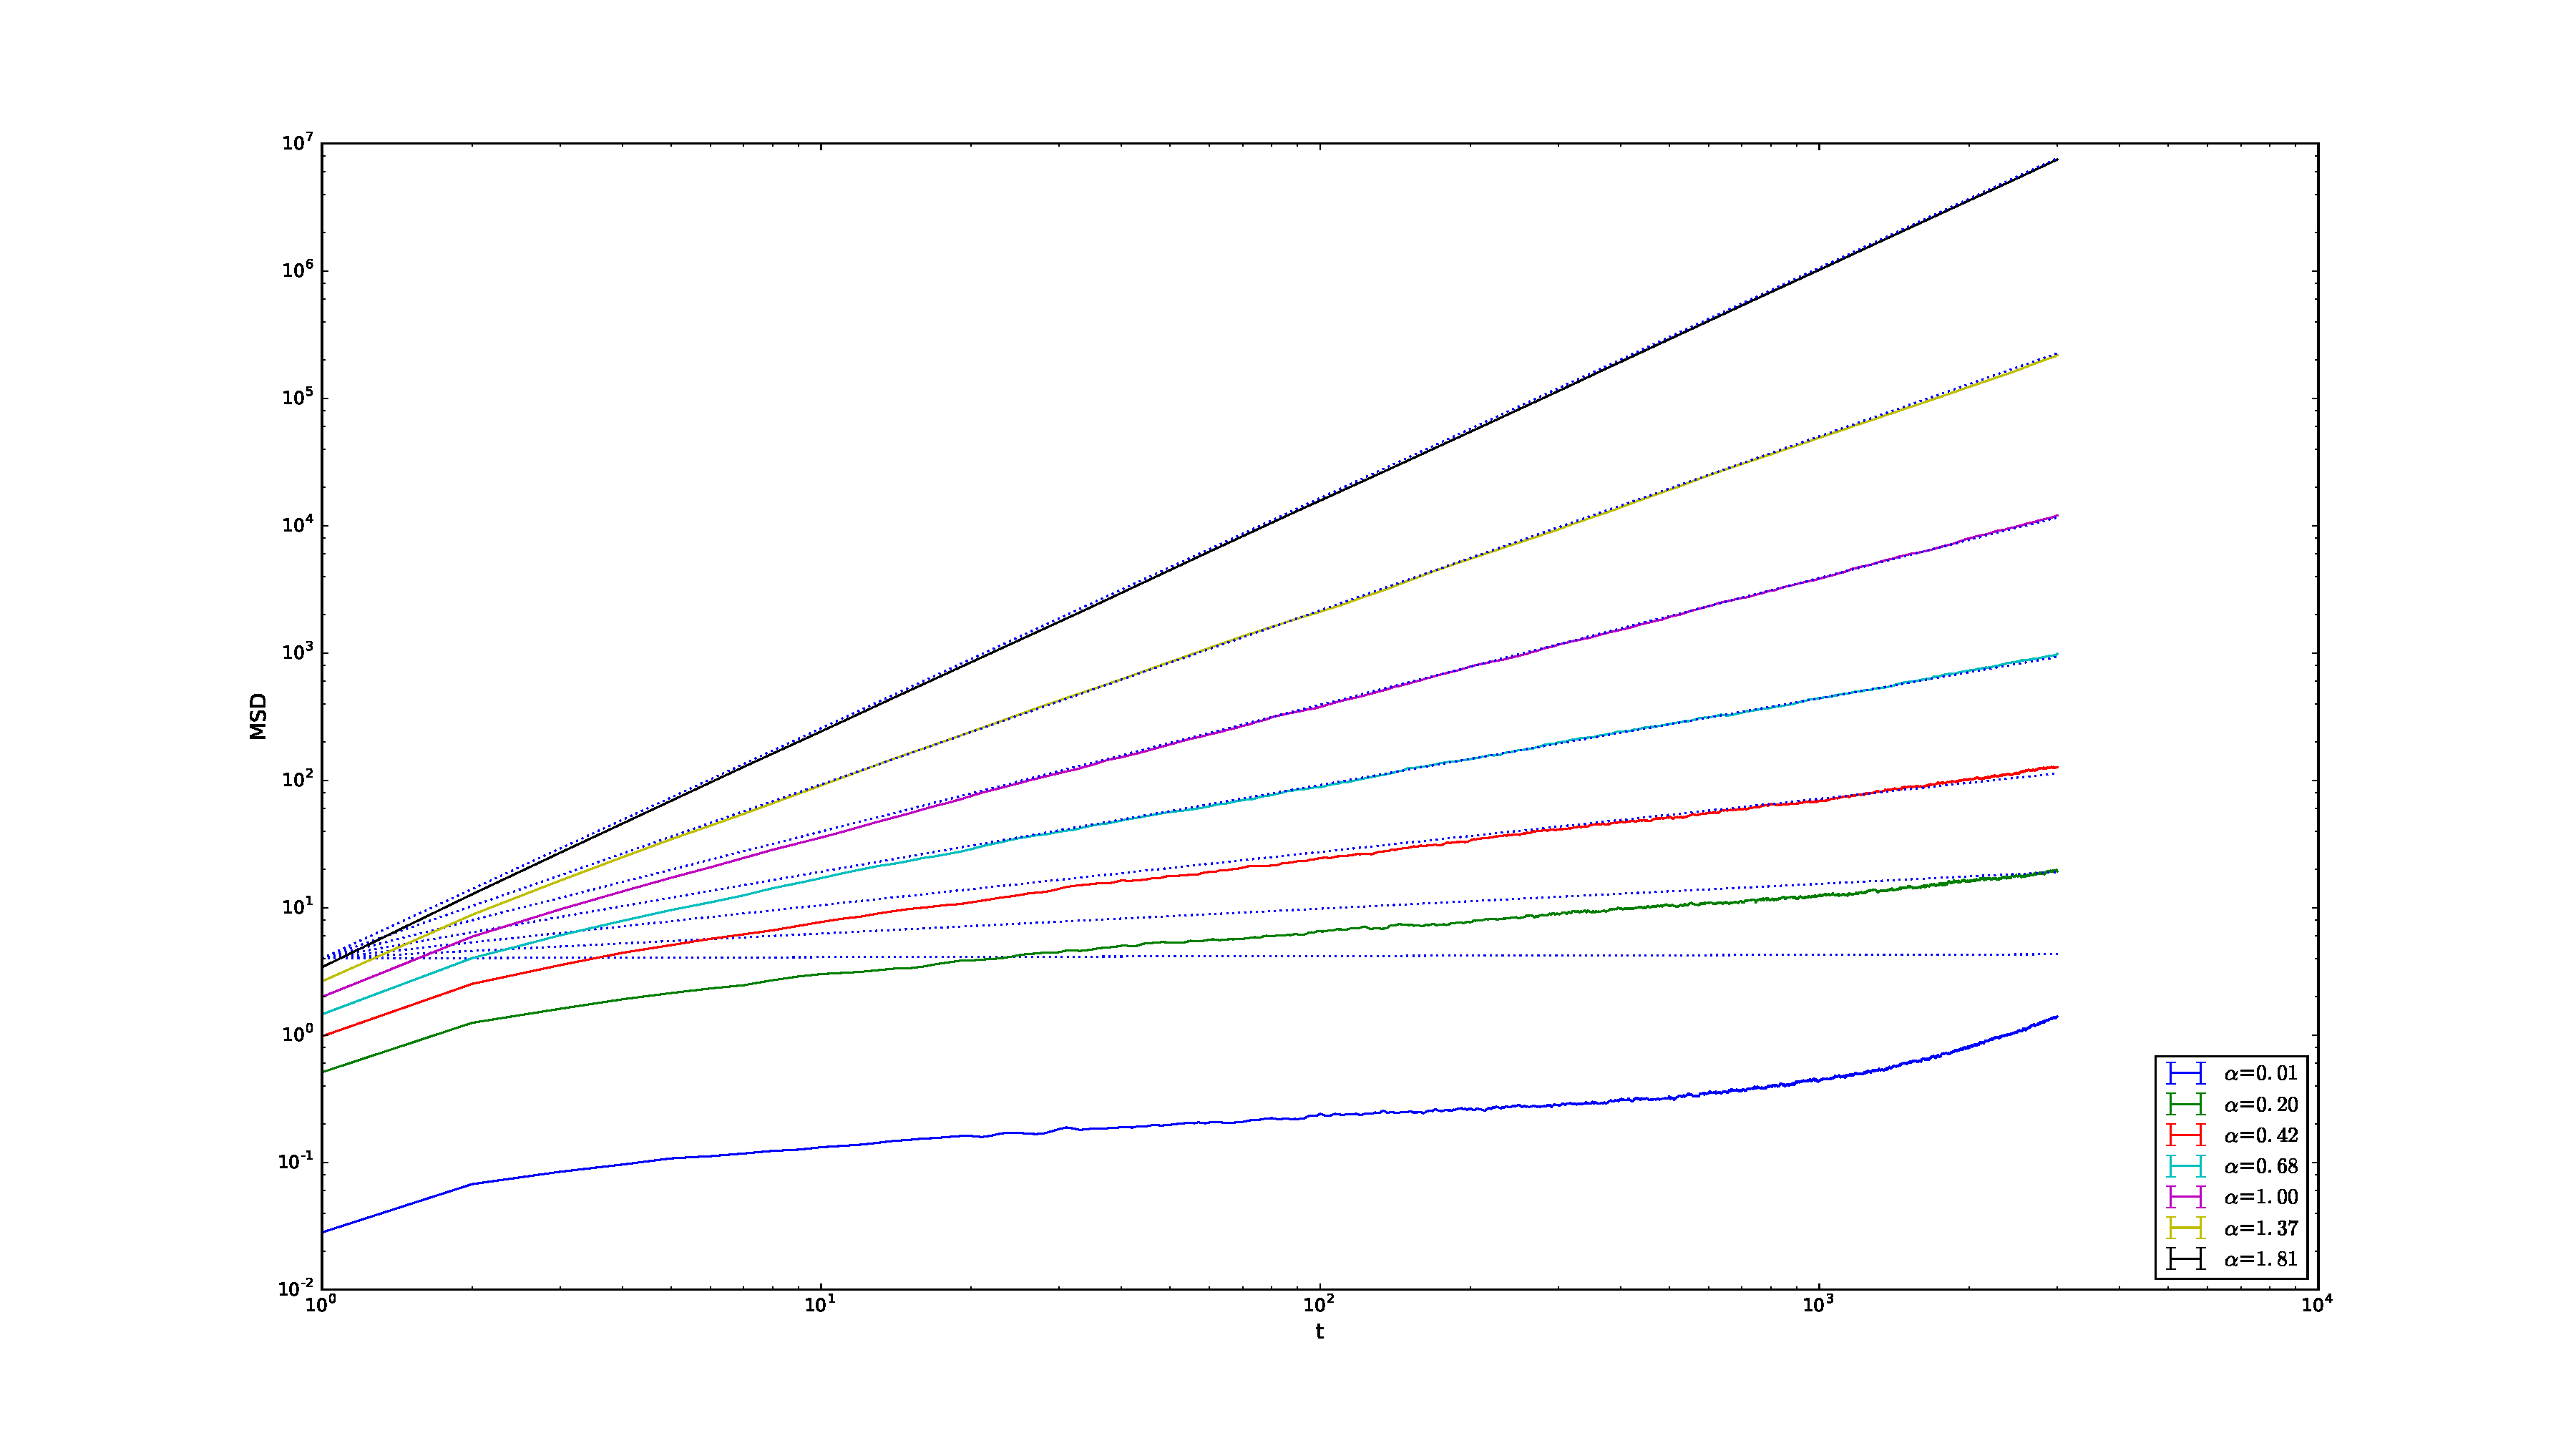
\includegraphics[width=\textwidth]{./msd_ensemble_alpha.pdf}
\caption{Mean Square Displacement of different $\alpha$}
% msd_ensemble_4000particles_log.pdf: 0x0 pixel, -2147483648dpi, 0.00x0.00 cm, bb=
 \centering
\end{figure}


\begin{figure}[h]
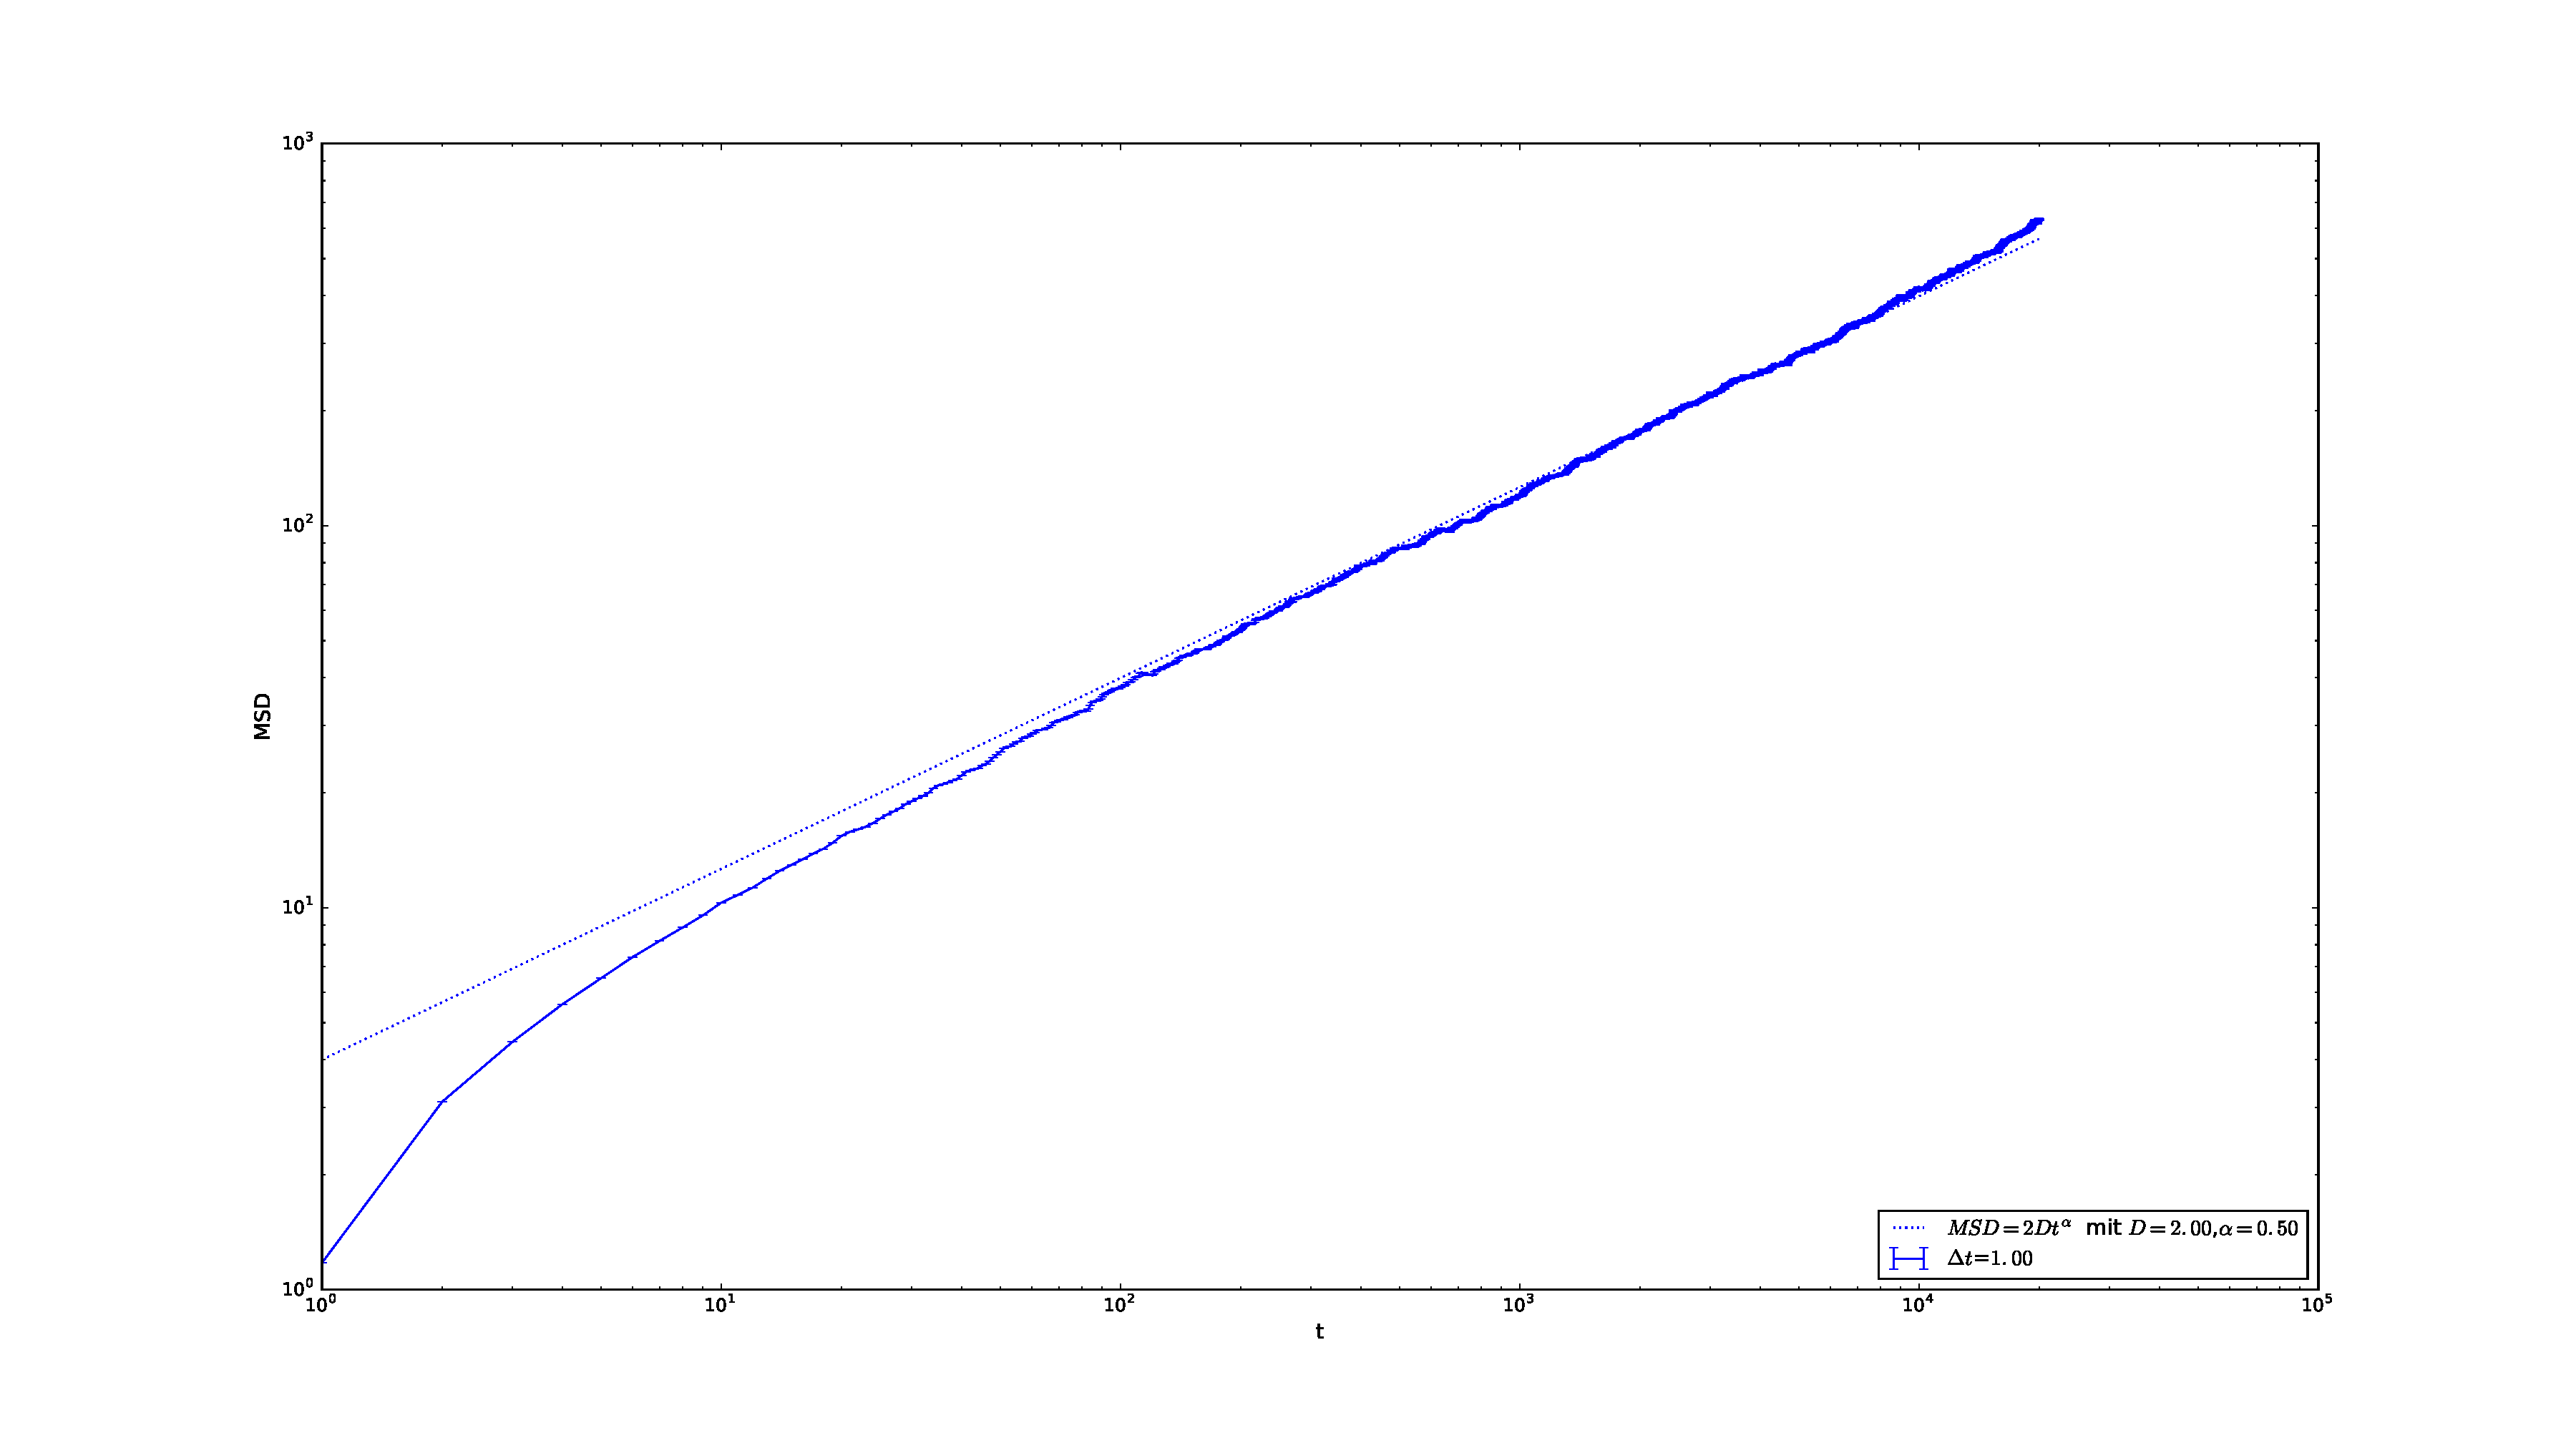
\includegraphics[width=\textwidth]{./msd_ensemble_4000particles_log.pdf}
\caption{Mean Square Displacement (Ensemble average of 4000 Trajectories)}
% msd_ensemble_4000particles_log.pdf: 0x0 pixel, -2147483648dpi, 0.00x0.00 cm, bb=
 \centering
\end{figure}

\begin{figure}[h]
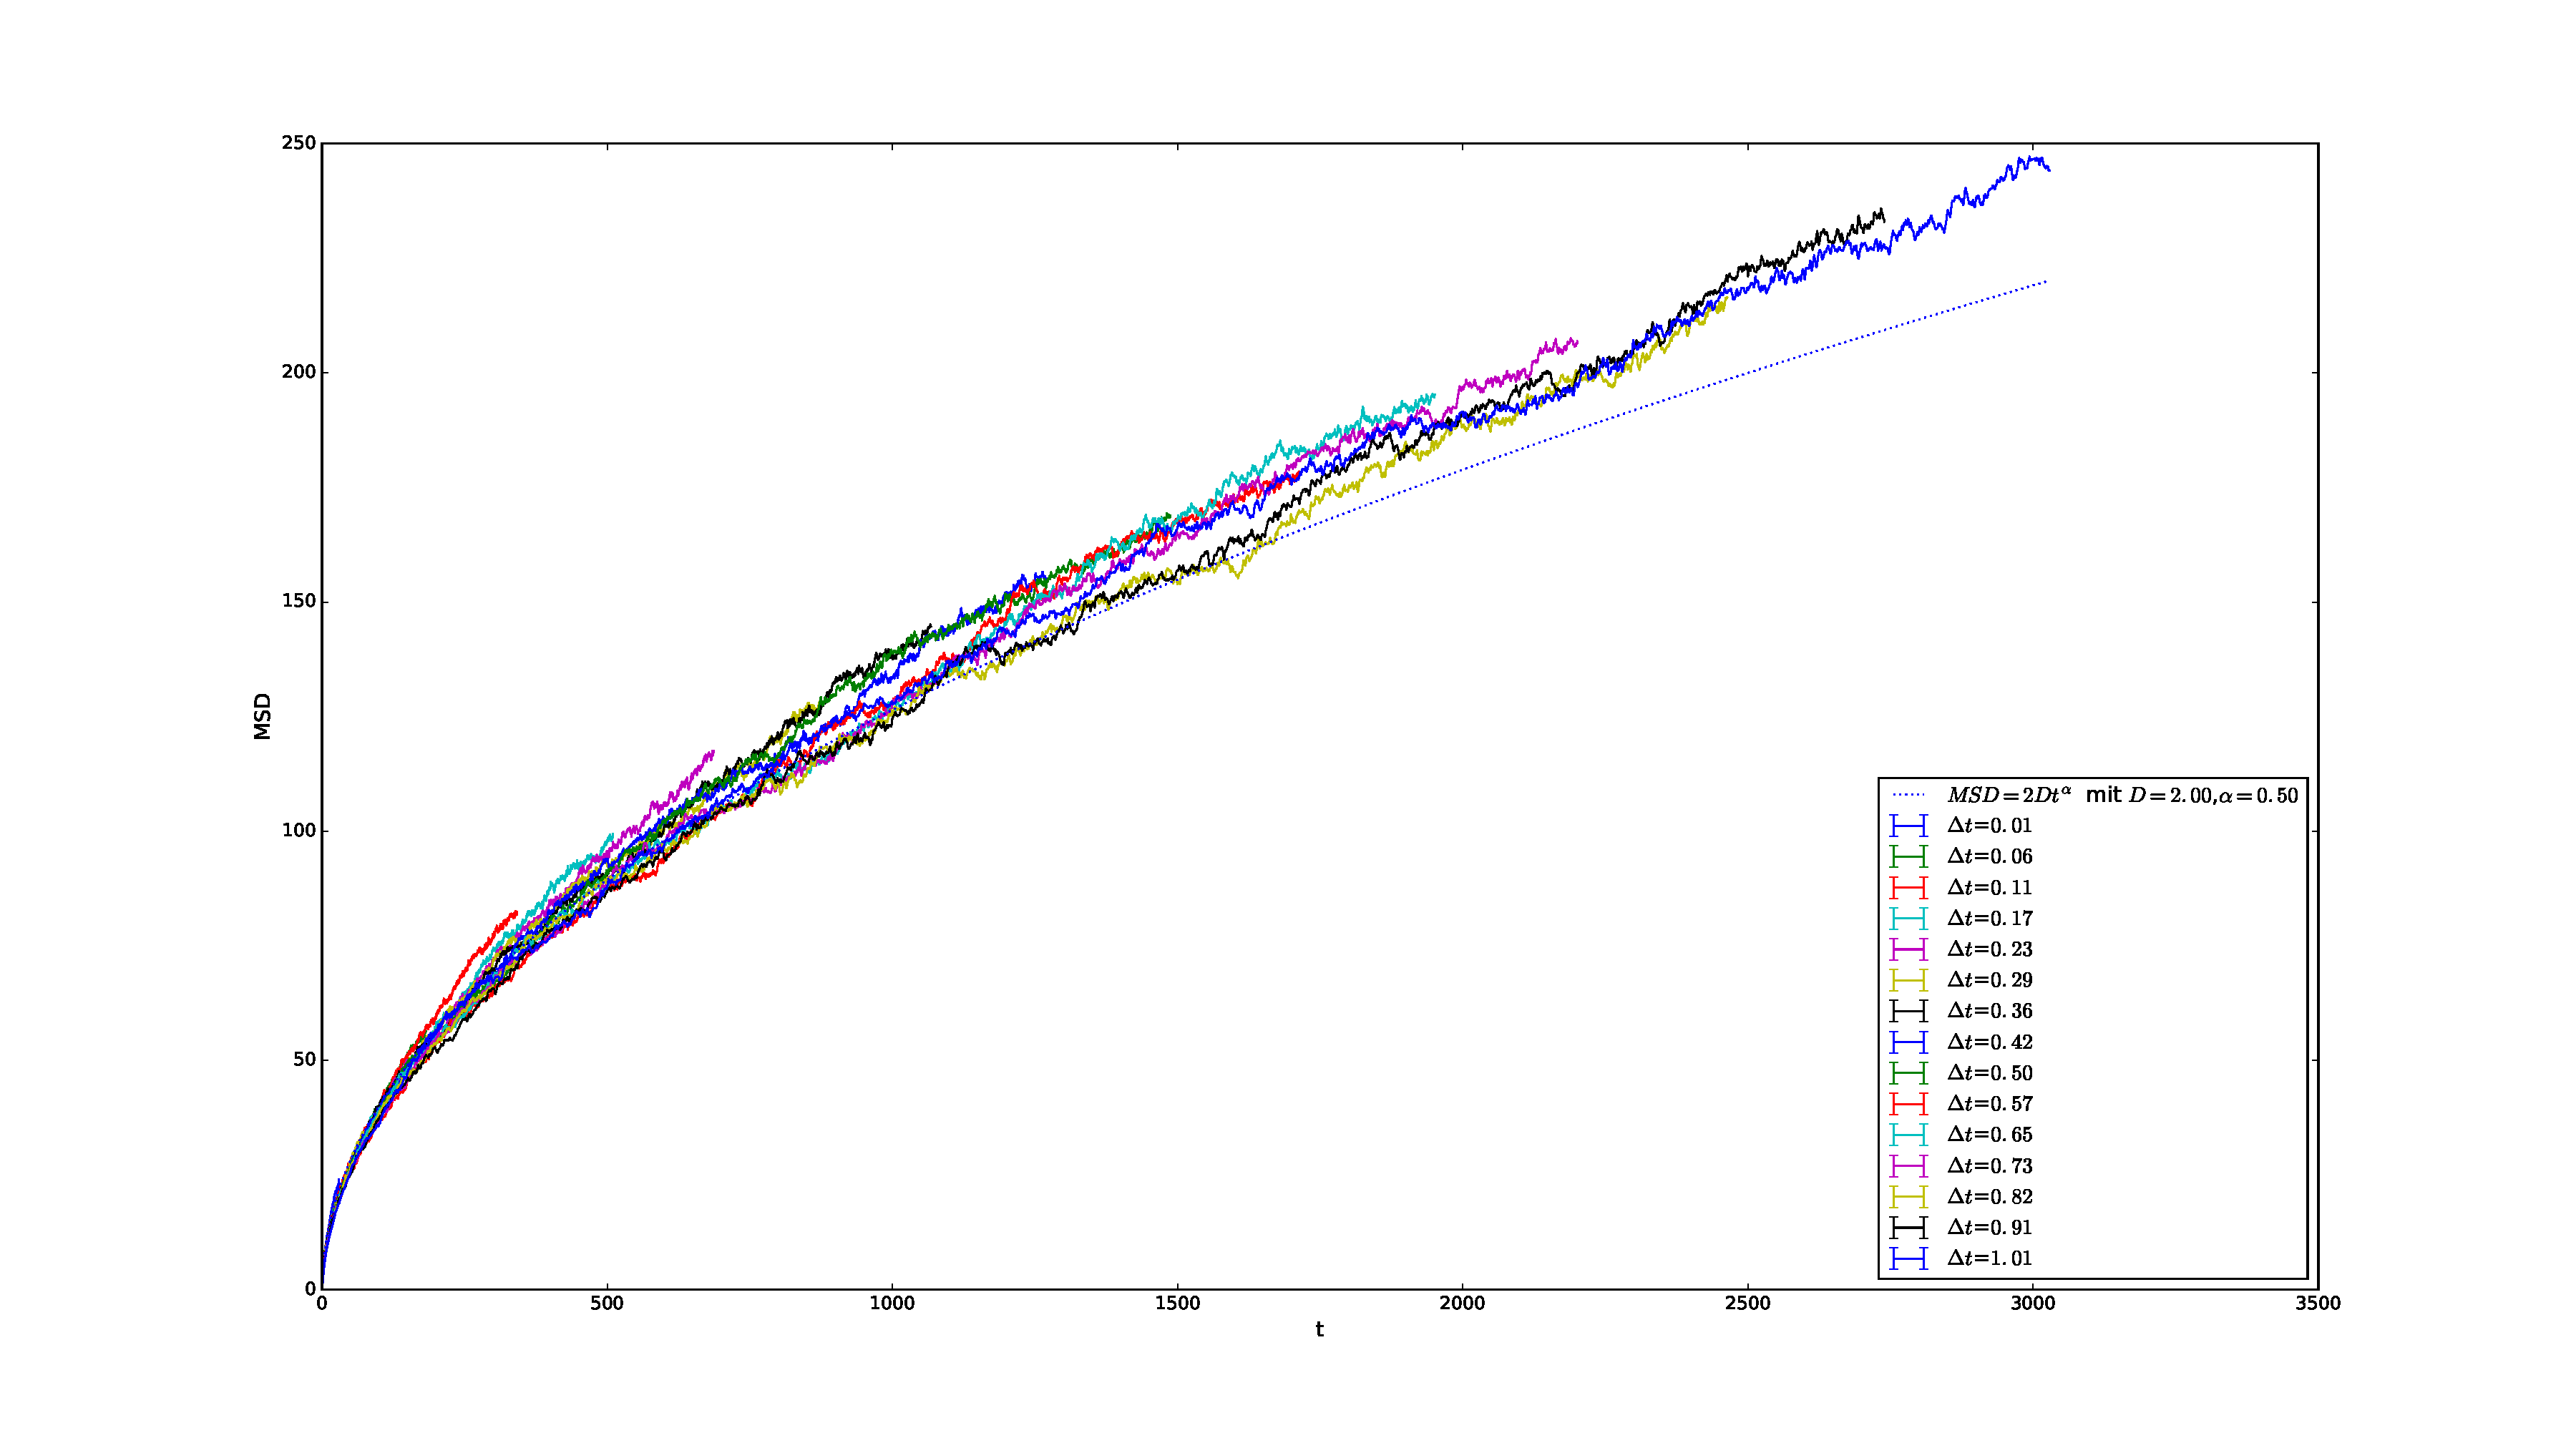
\includegraphics[width=\textwidth]{./msd_ensemble_dt_nostd_lin.pdf}
\caption{Mean Square Displacement (Ensemble average fpr different $\Delta t$)}
% msd_ensemble_4000particles_log.pdf: 0x0 pixel, -2147483648dpi, 0.00x0.00 cm, bb=
 \centering
\end{figure}

\begin{figure}[h]
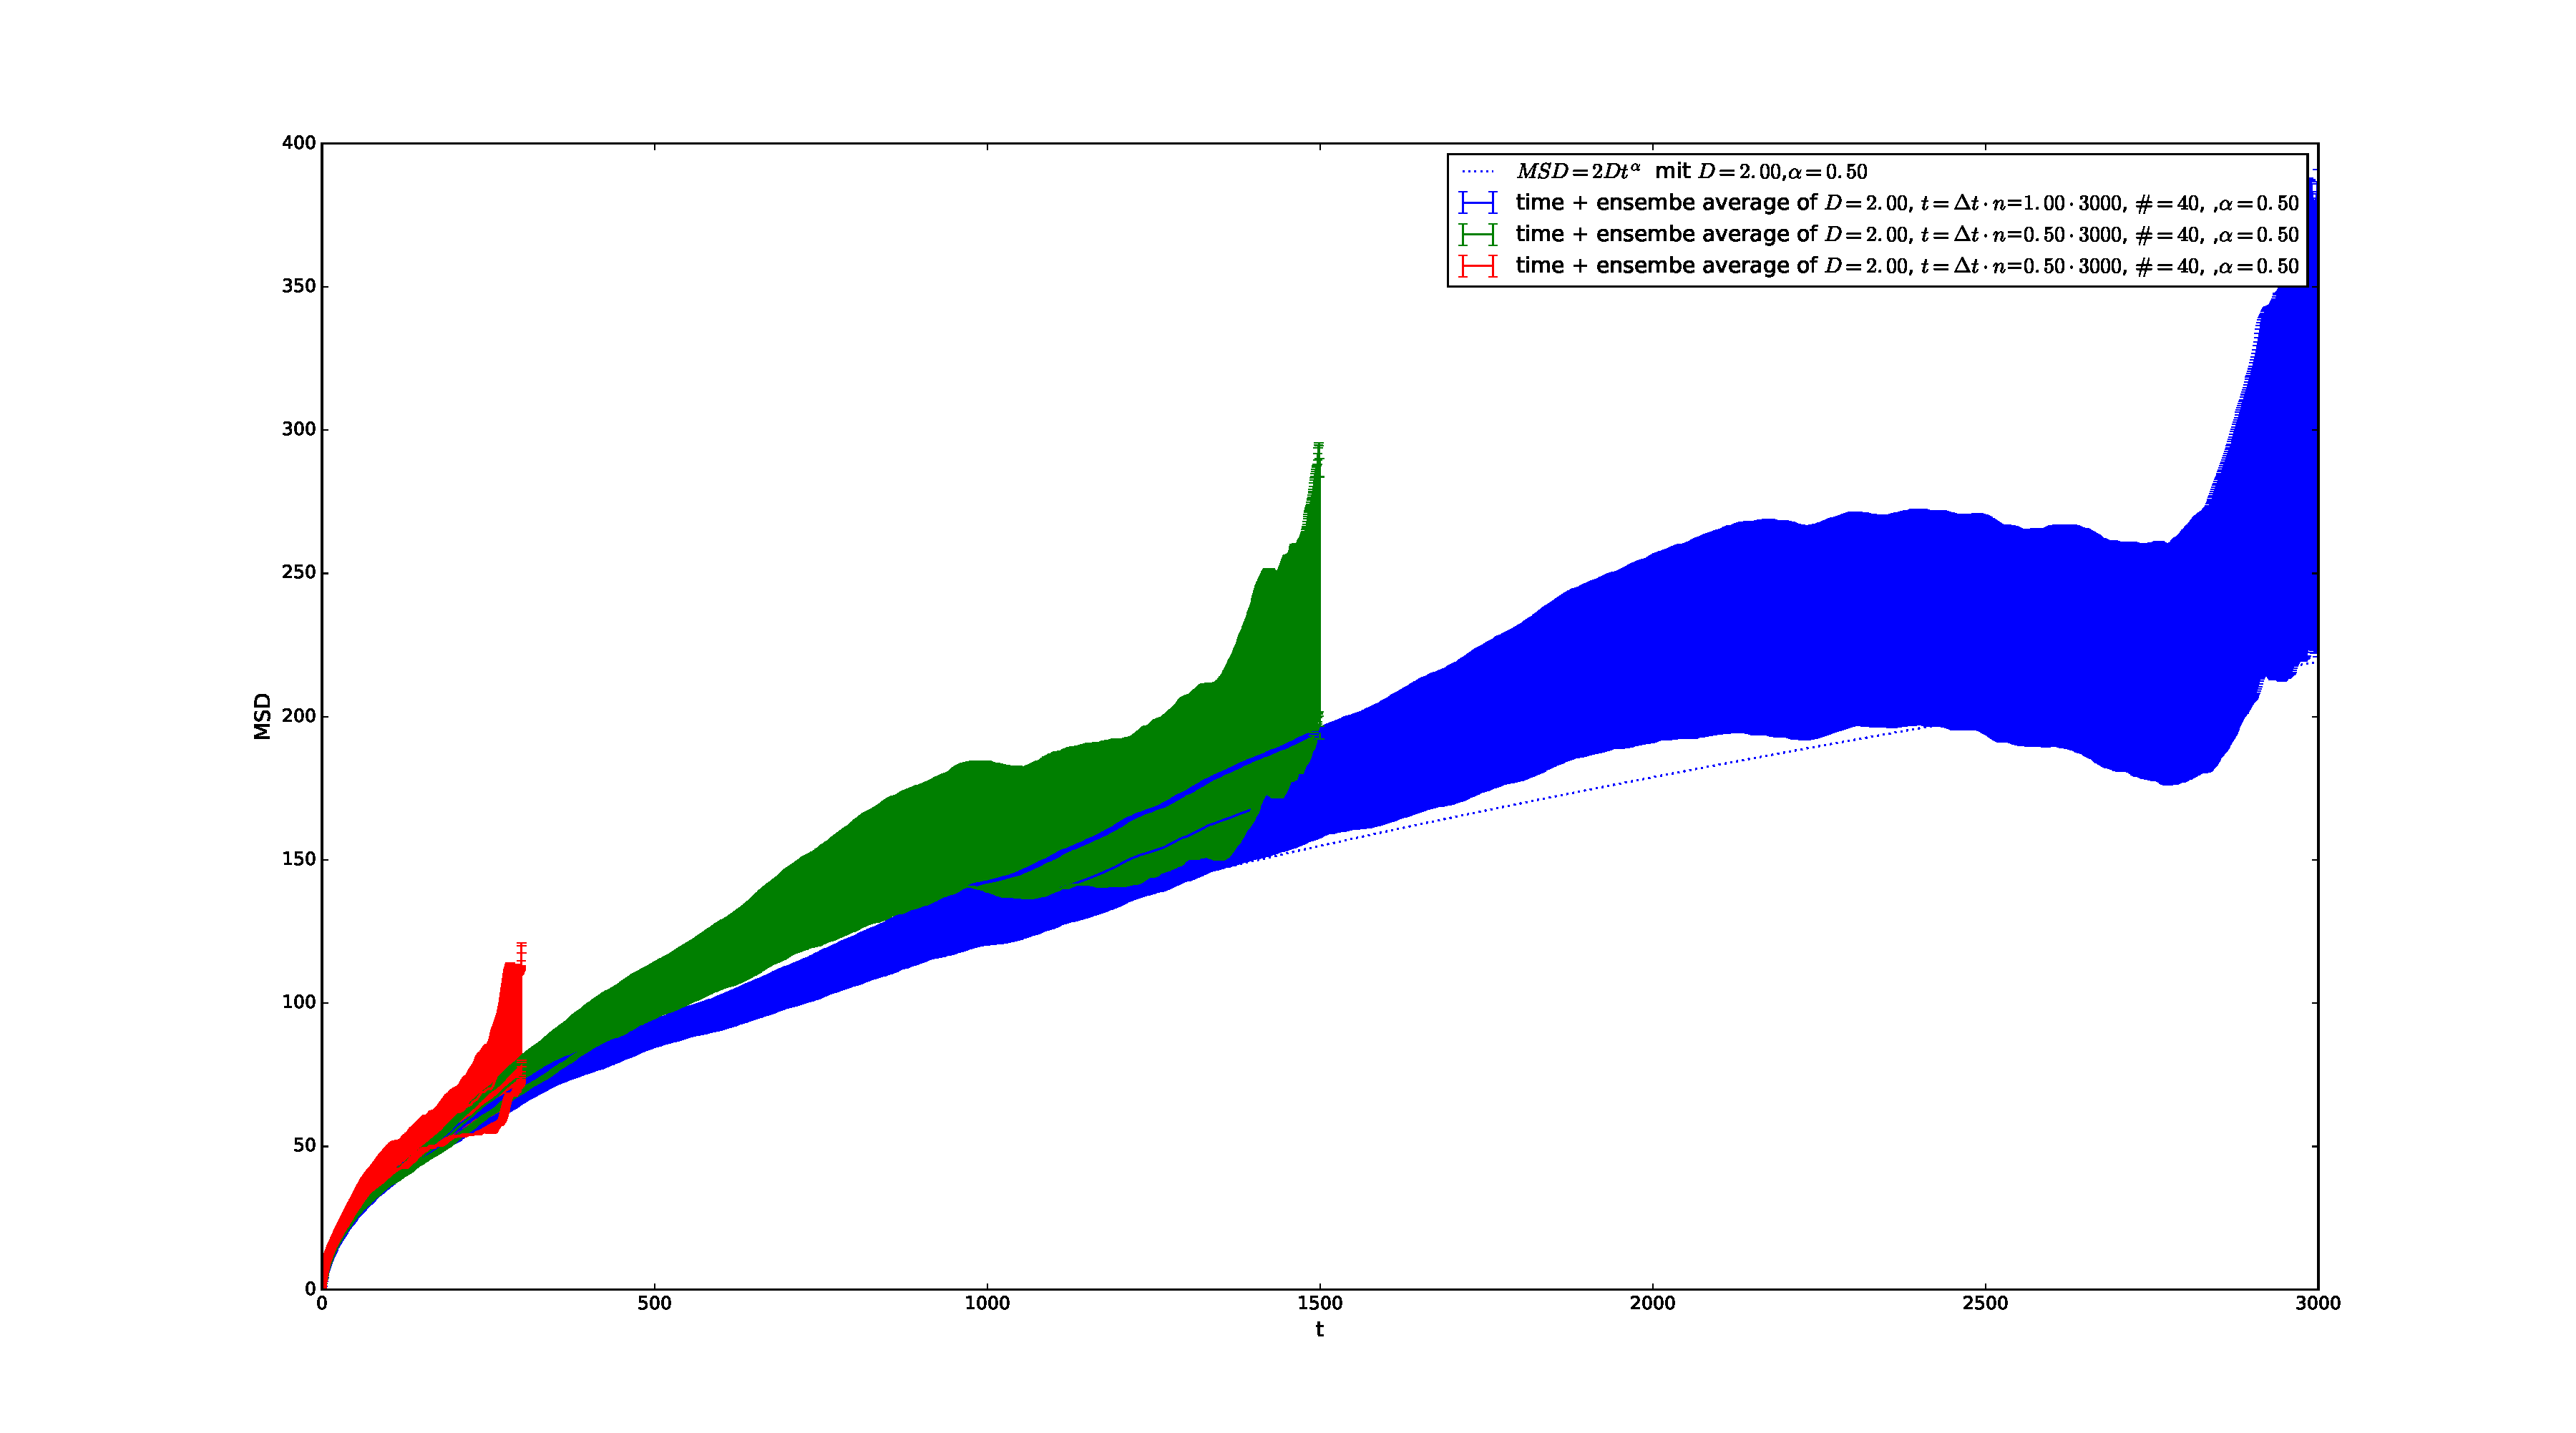
\includegraphics[width=\textwidth]{./msd_time_ensemble_dt_lin.pdf}
\caption{Mean Square Displacement (time and ensemble avarge for different $ \Delta t$ and with standard deviation of the Mean)}
% msd_ensemble_4000particles_log.pdf: 0x0 pixel, -2147483648dpi, 0.00x0.00 cm, bb=
 \centering
\end{figure}

\begin{figure}[h]
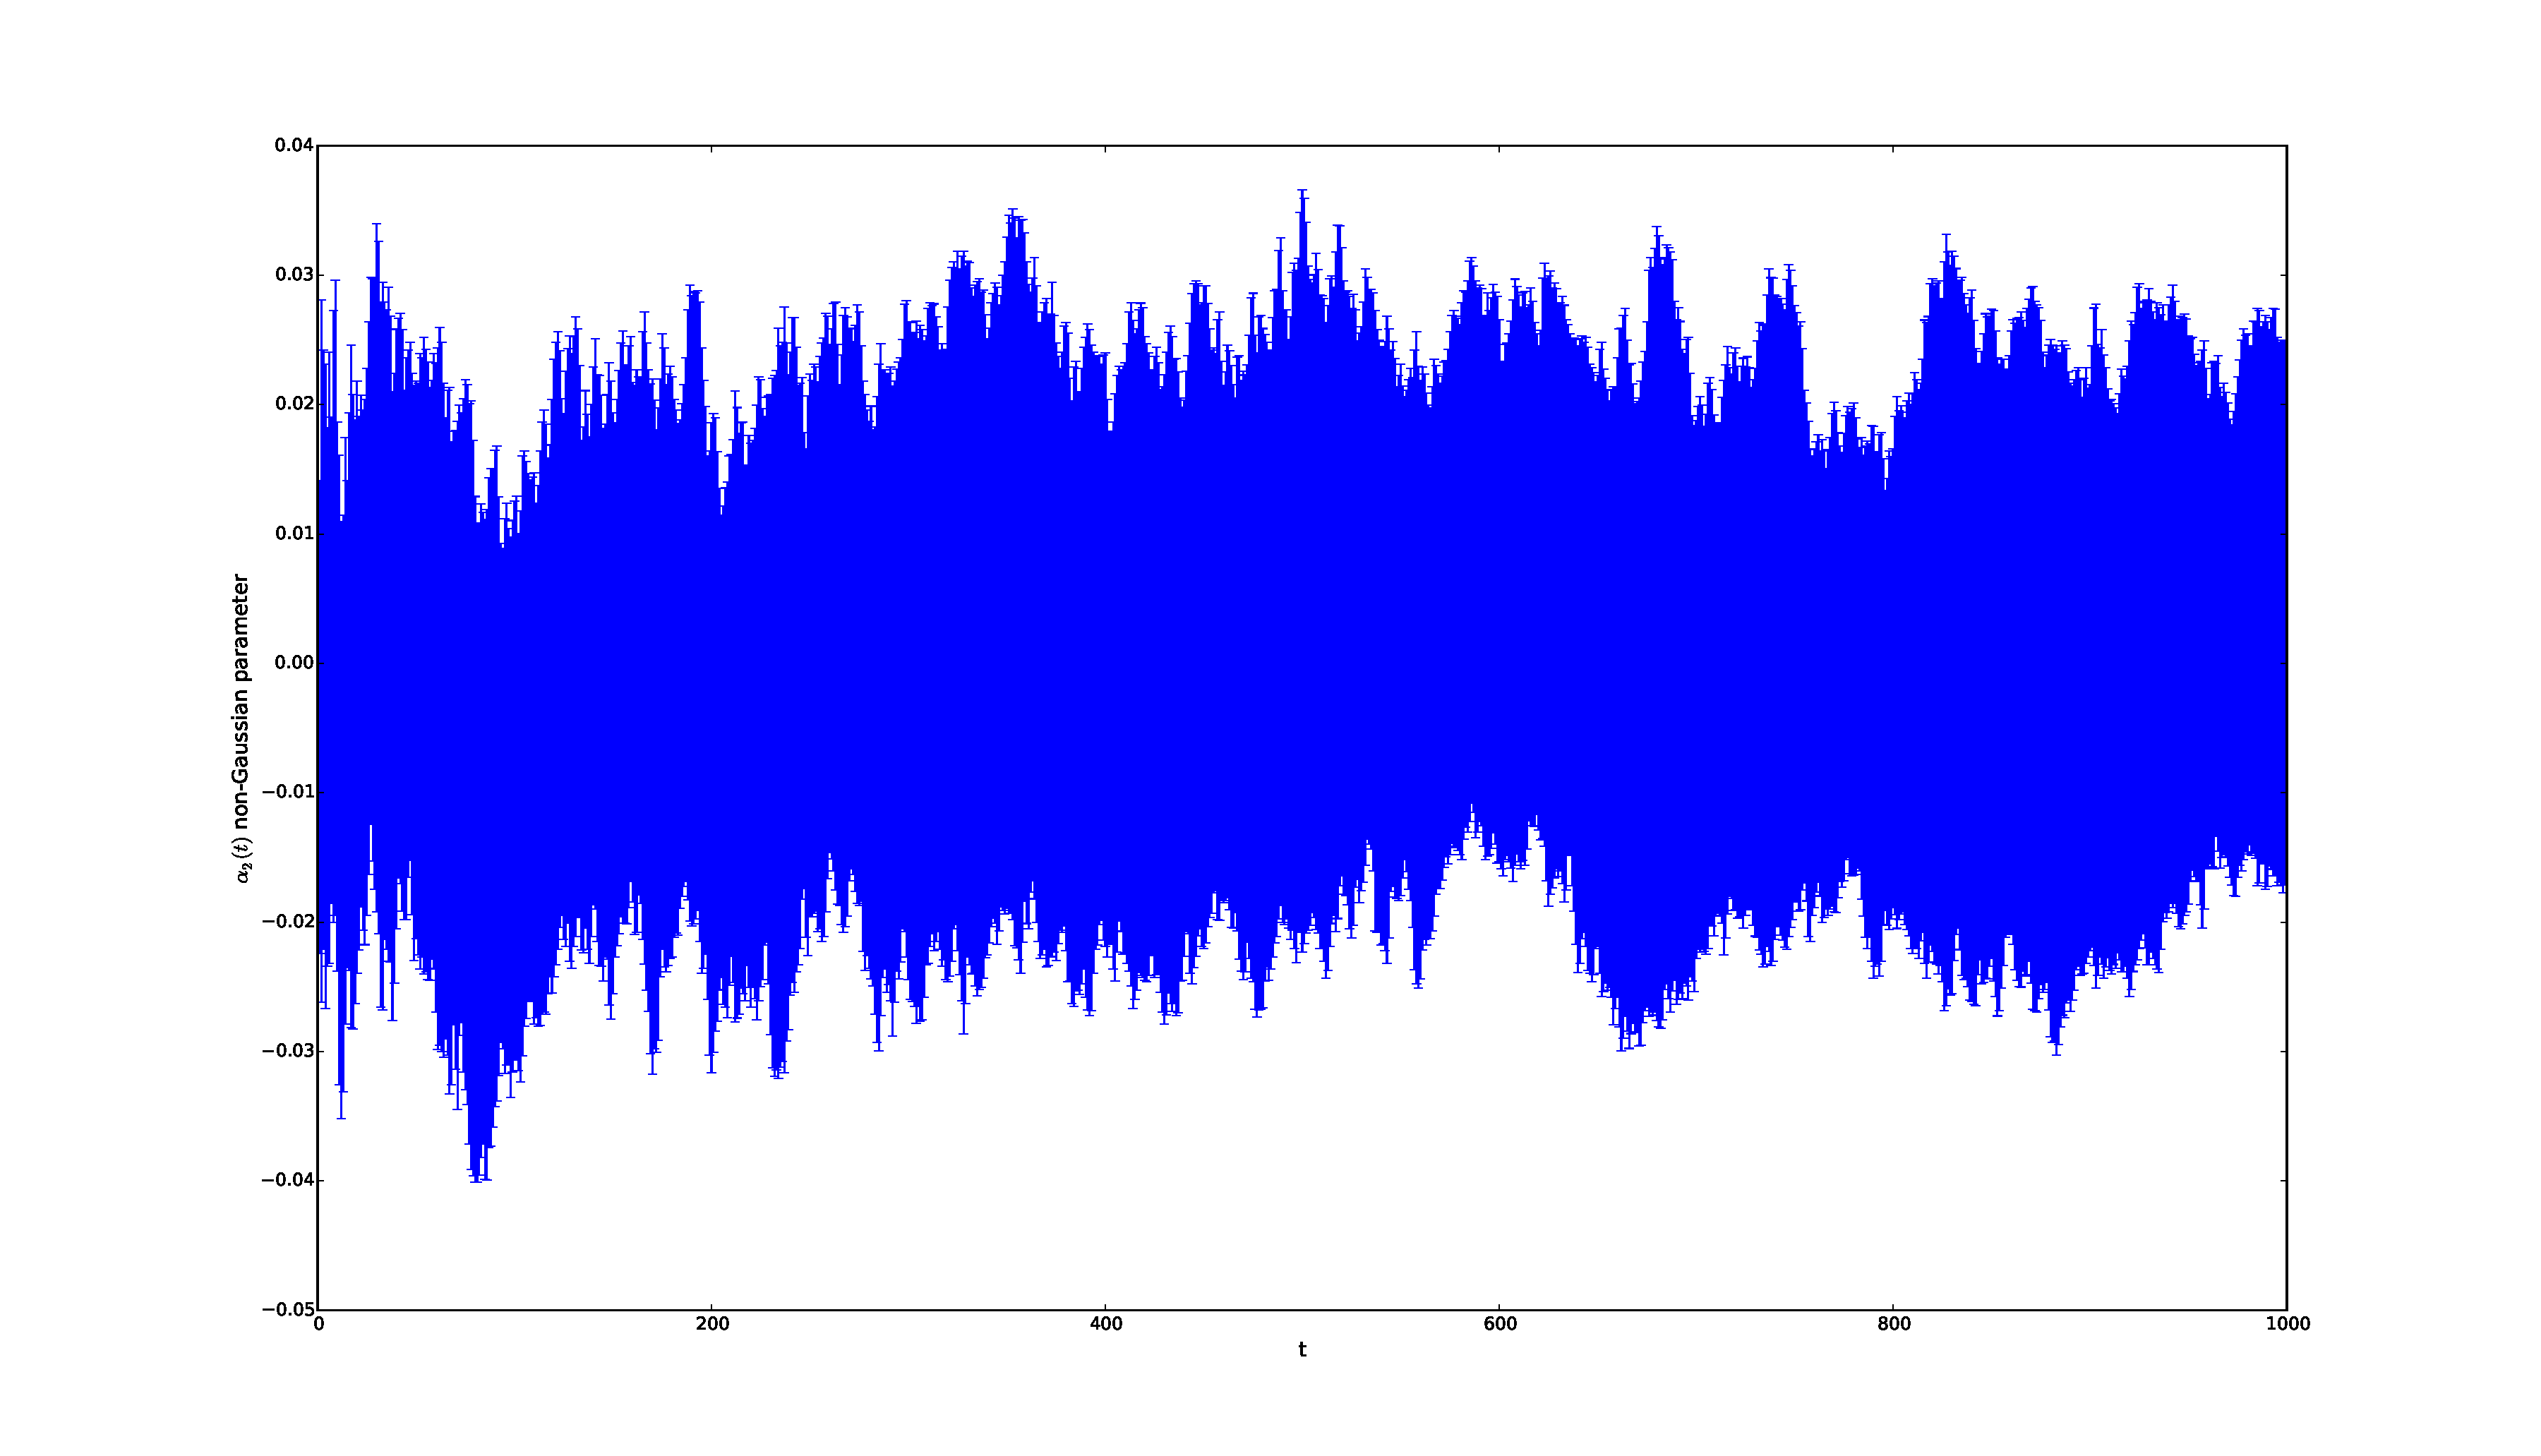
\includegraphics[width=\textwidth]{./non_gaussian_D=2_t=1001_dt=1_alpha=05particles_5000_std01.pdf}
\caption{Non-gaussian parameter of $\alpha=0.5$ , $ D=2 $ and 5000 trajectories ensemble.}
% msd_ensemble_4000particles_log.pdf: 0x0 pixel, -2147483648dpi, 0.00x0.00 cm, bb=
 \centering
\end{figure}

\begin{figure}[h]
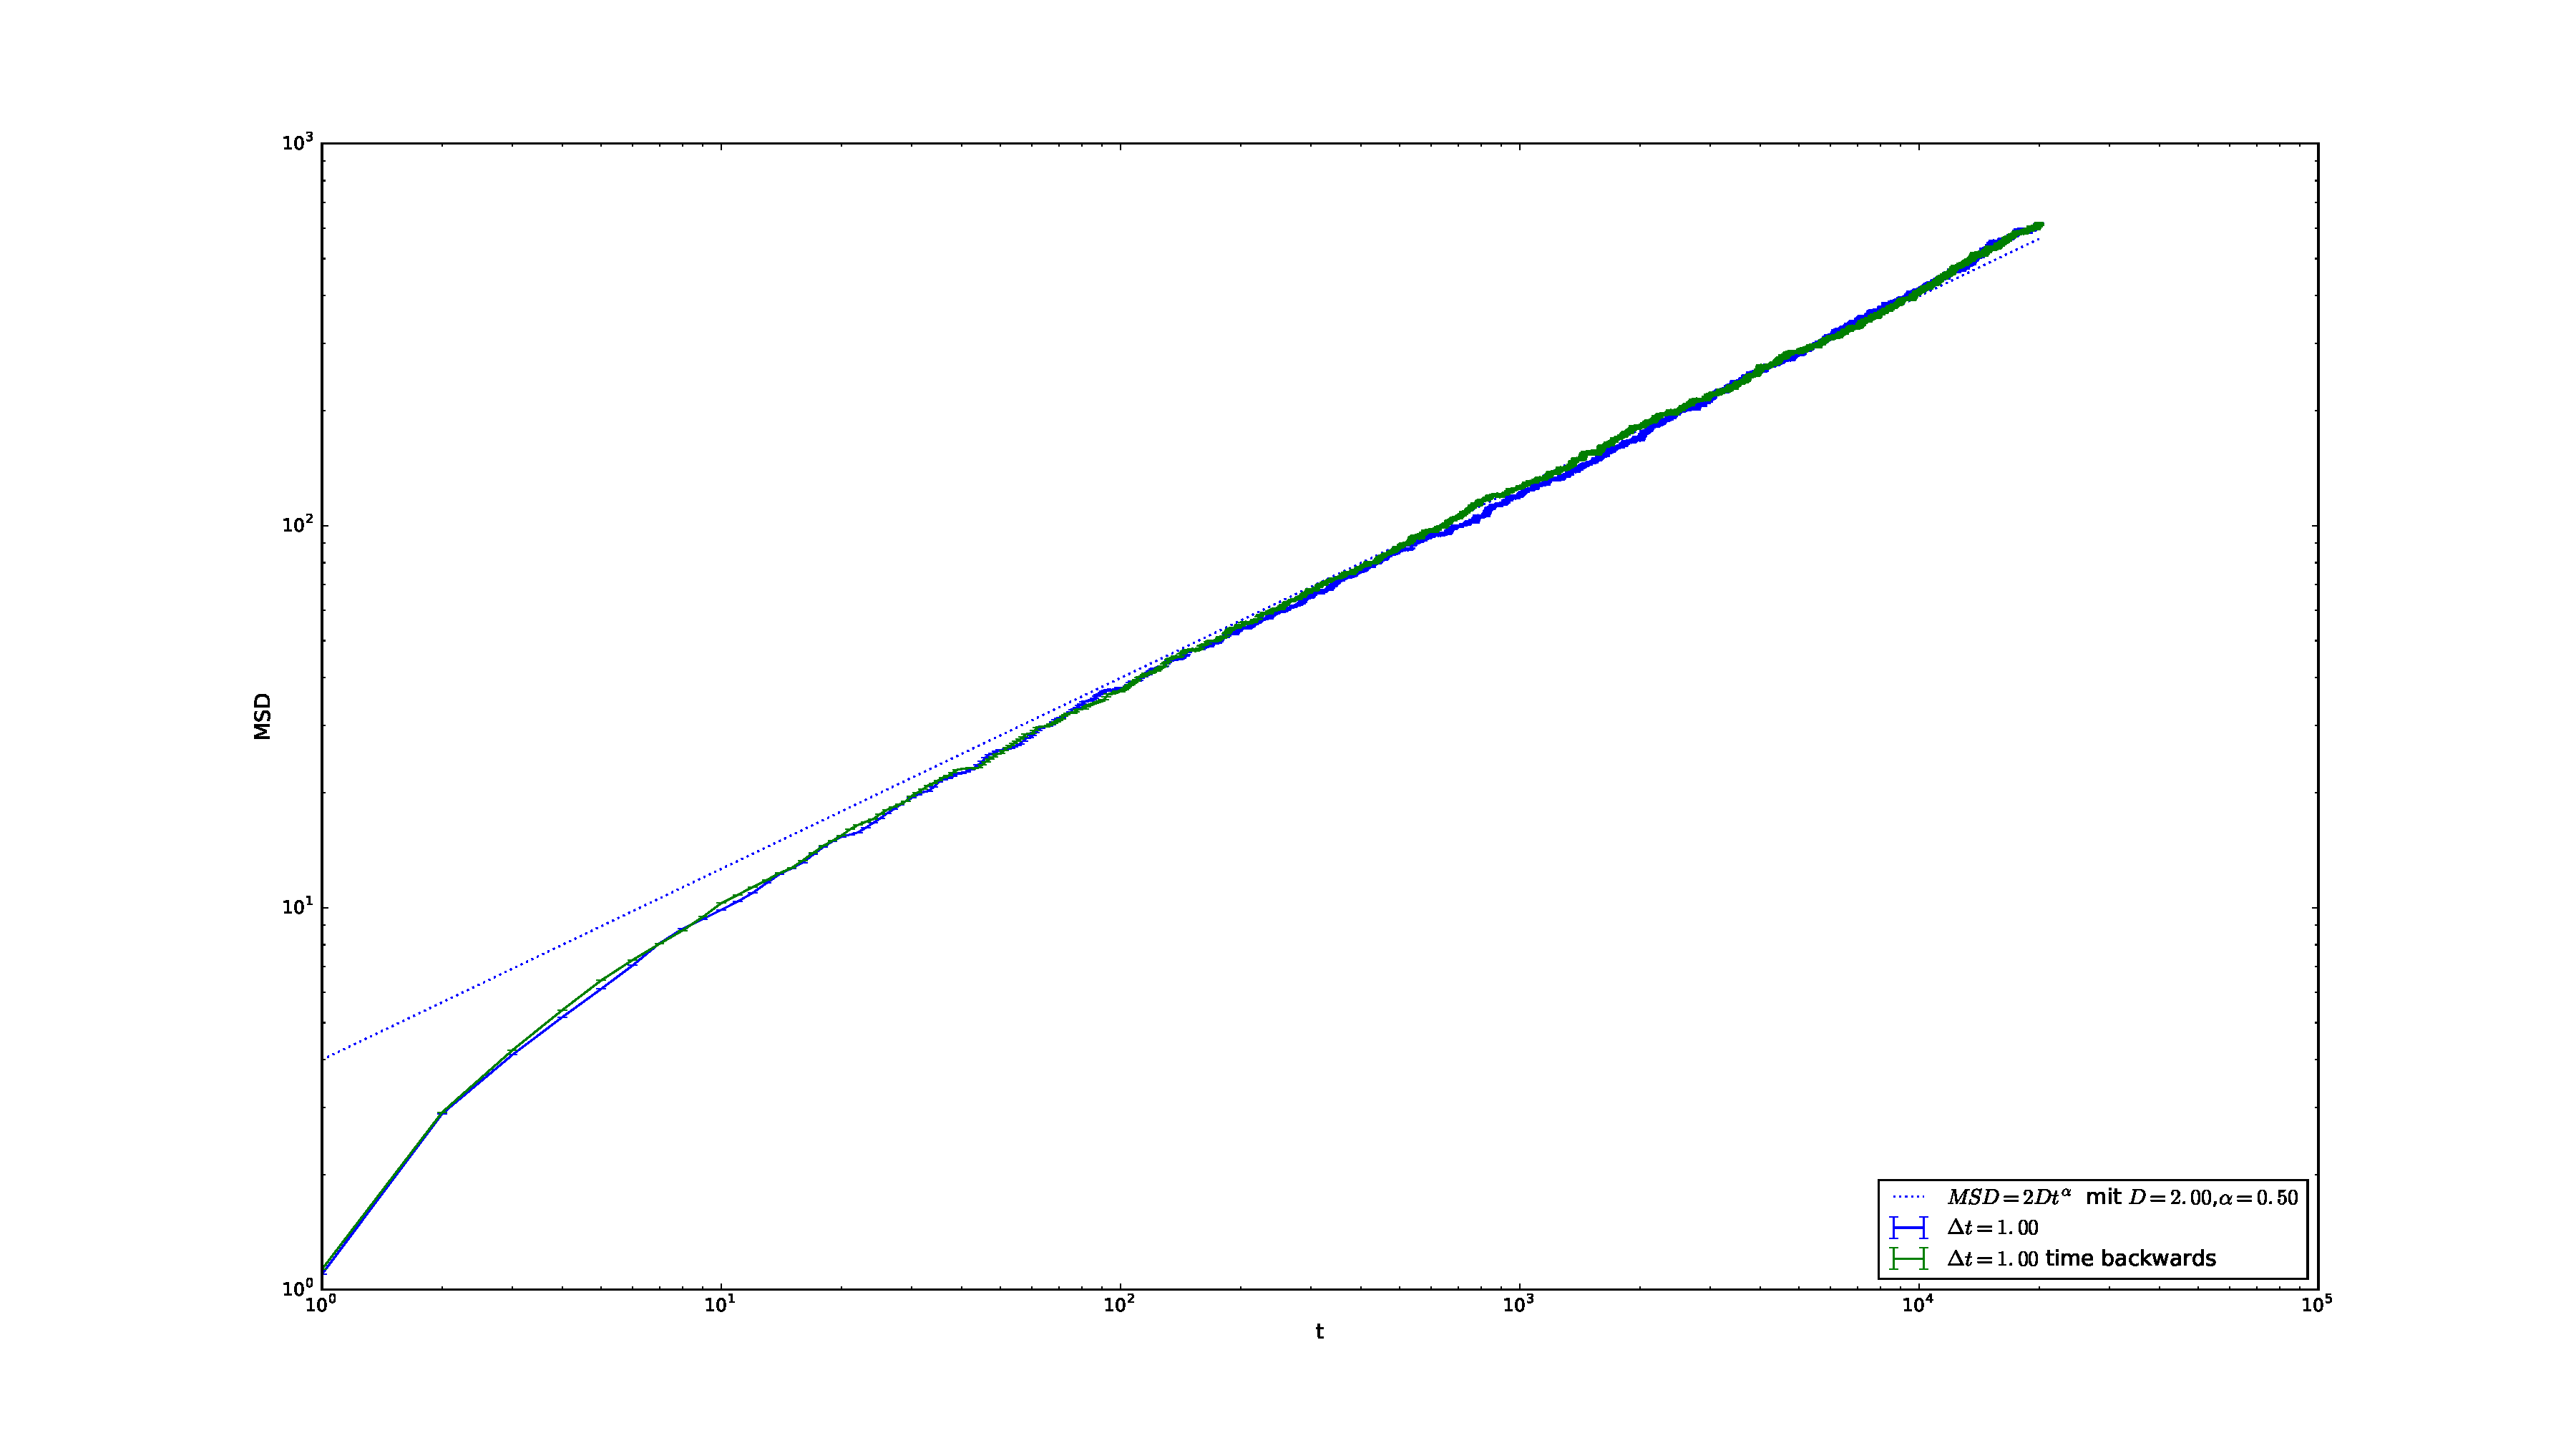
\includegraphics[width=\textwidth]{./msd_ensemble_t_inverted.pdf}
\caption{Non-gaussian parameter of $\alpha=0.5$ , $ D=2 $ and 5000 trajectories ensemble.}
% msd_ensemble_4000particles_log.pdf: 0x0 pixel, -2147483648dpi, 0.00x0.00 cm, bb=
 \centering
\end{figure}

\begin{figure}[h]
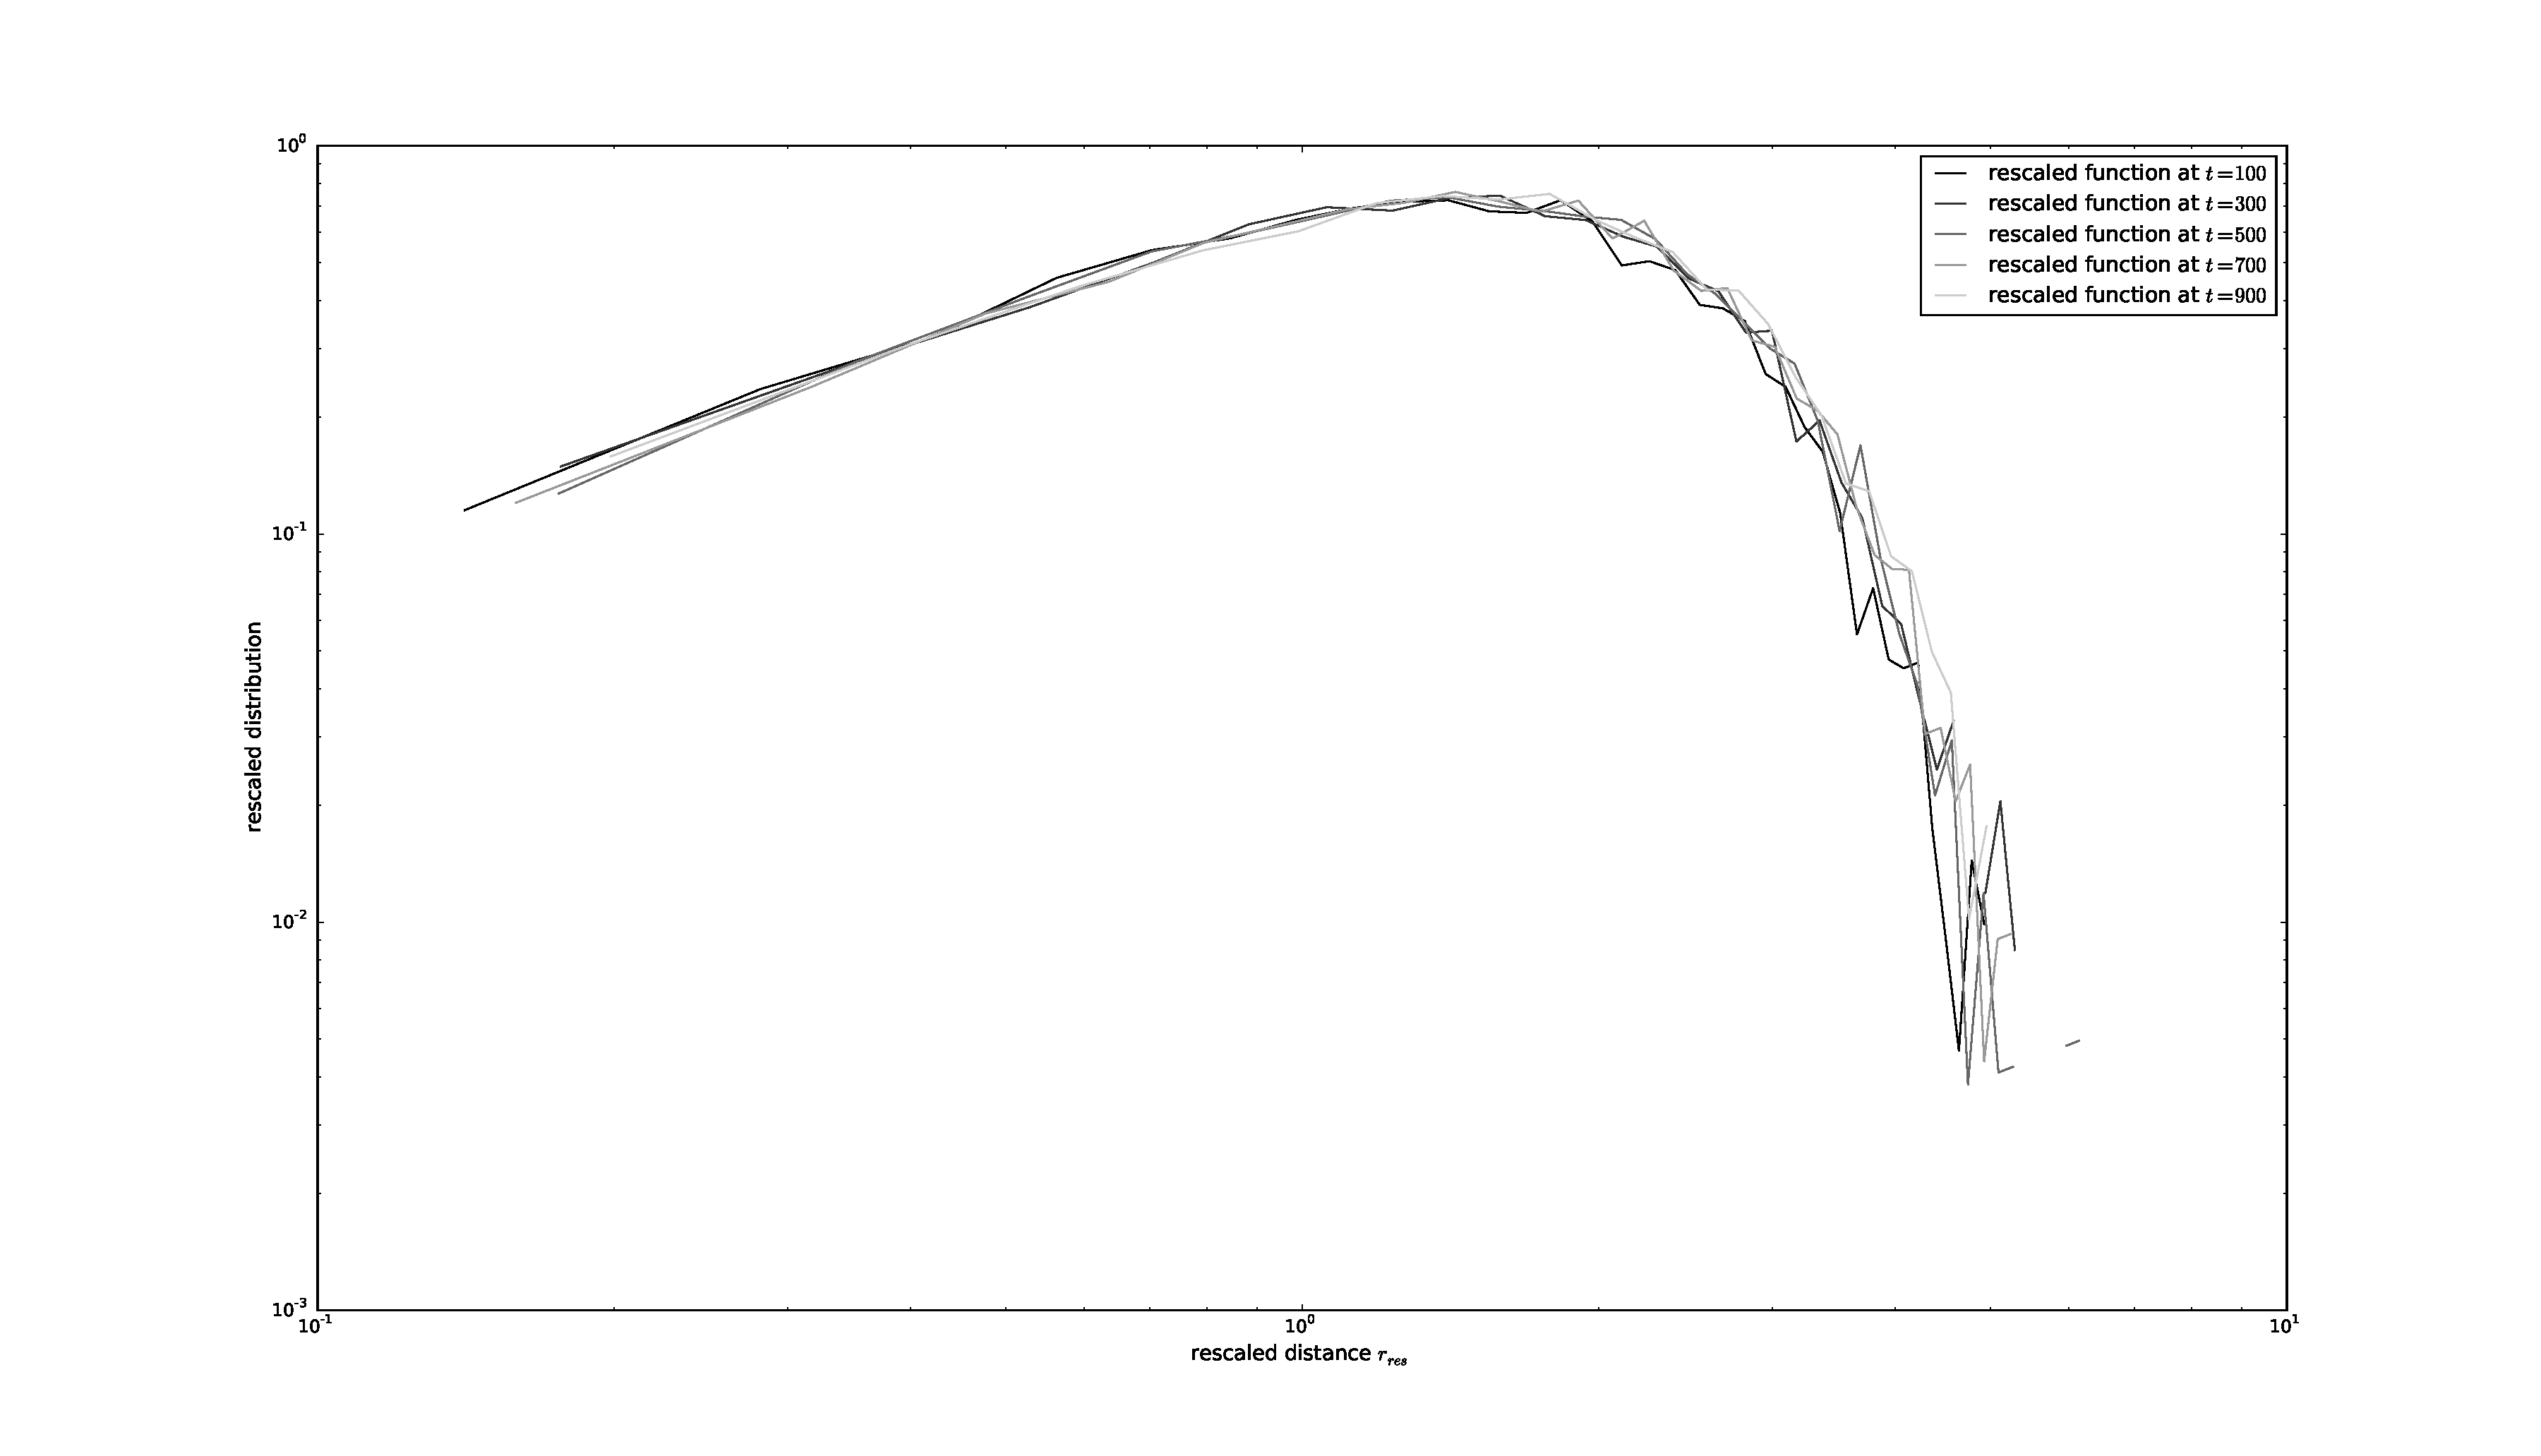
\includegraphics[width=\textwidth]{./rescaled_function.pdf}
\caption{rescaled function for different times}
% msd_ensemble_4000particles_log.pdf: 0x0 pixel, -2147483648dpi, 0.00x0.00 cm, bb=
 \centering
\end{figure}

\begin{figure}[h]
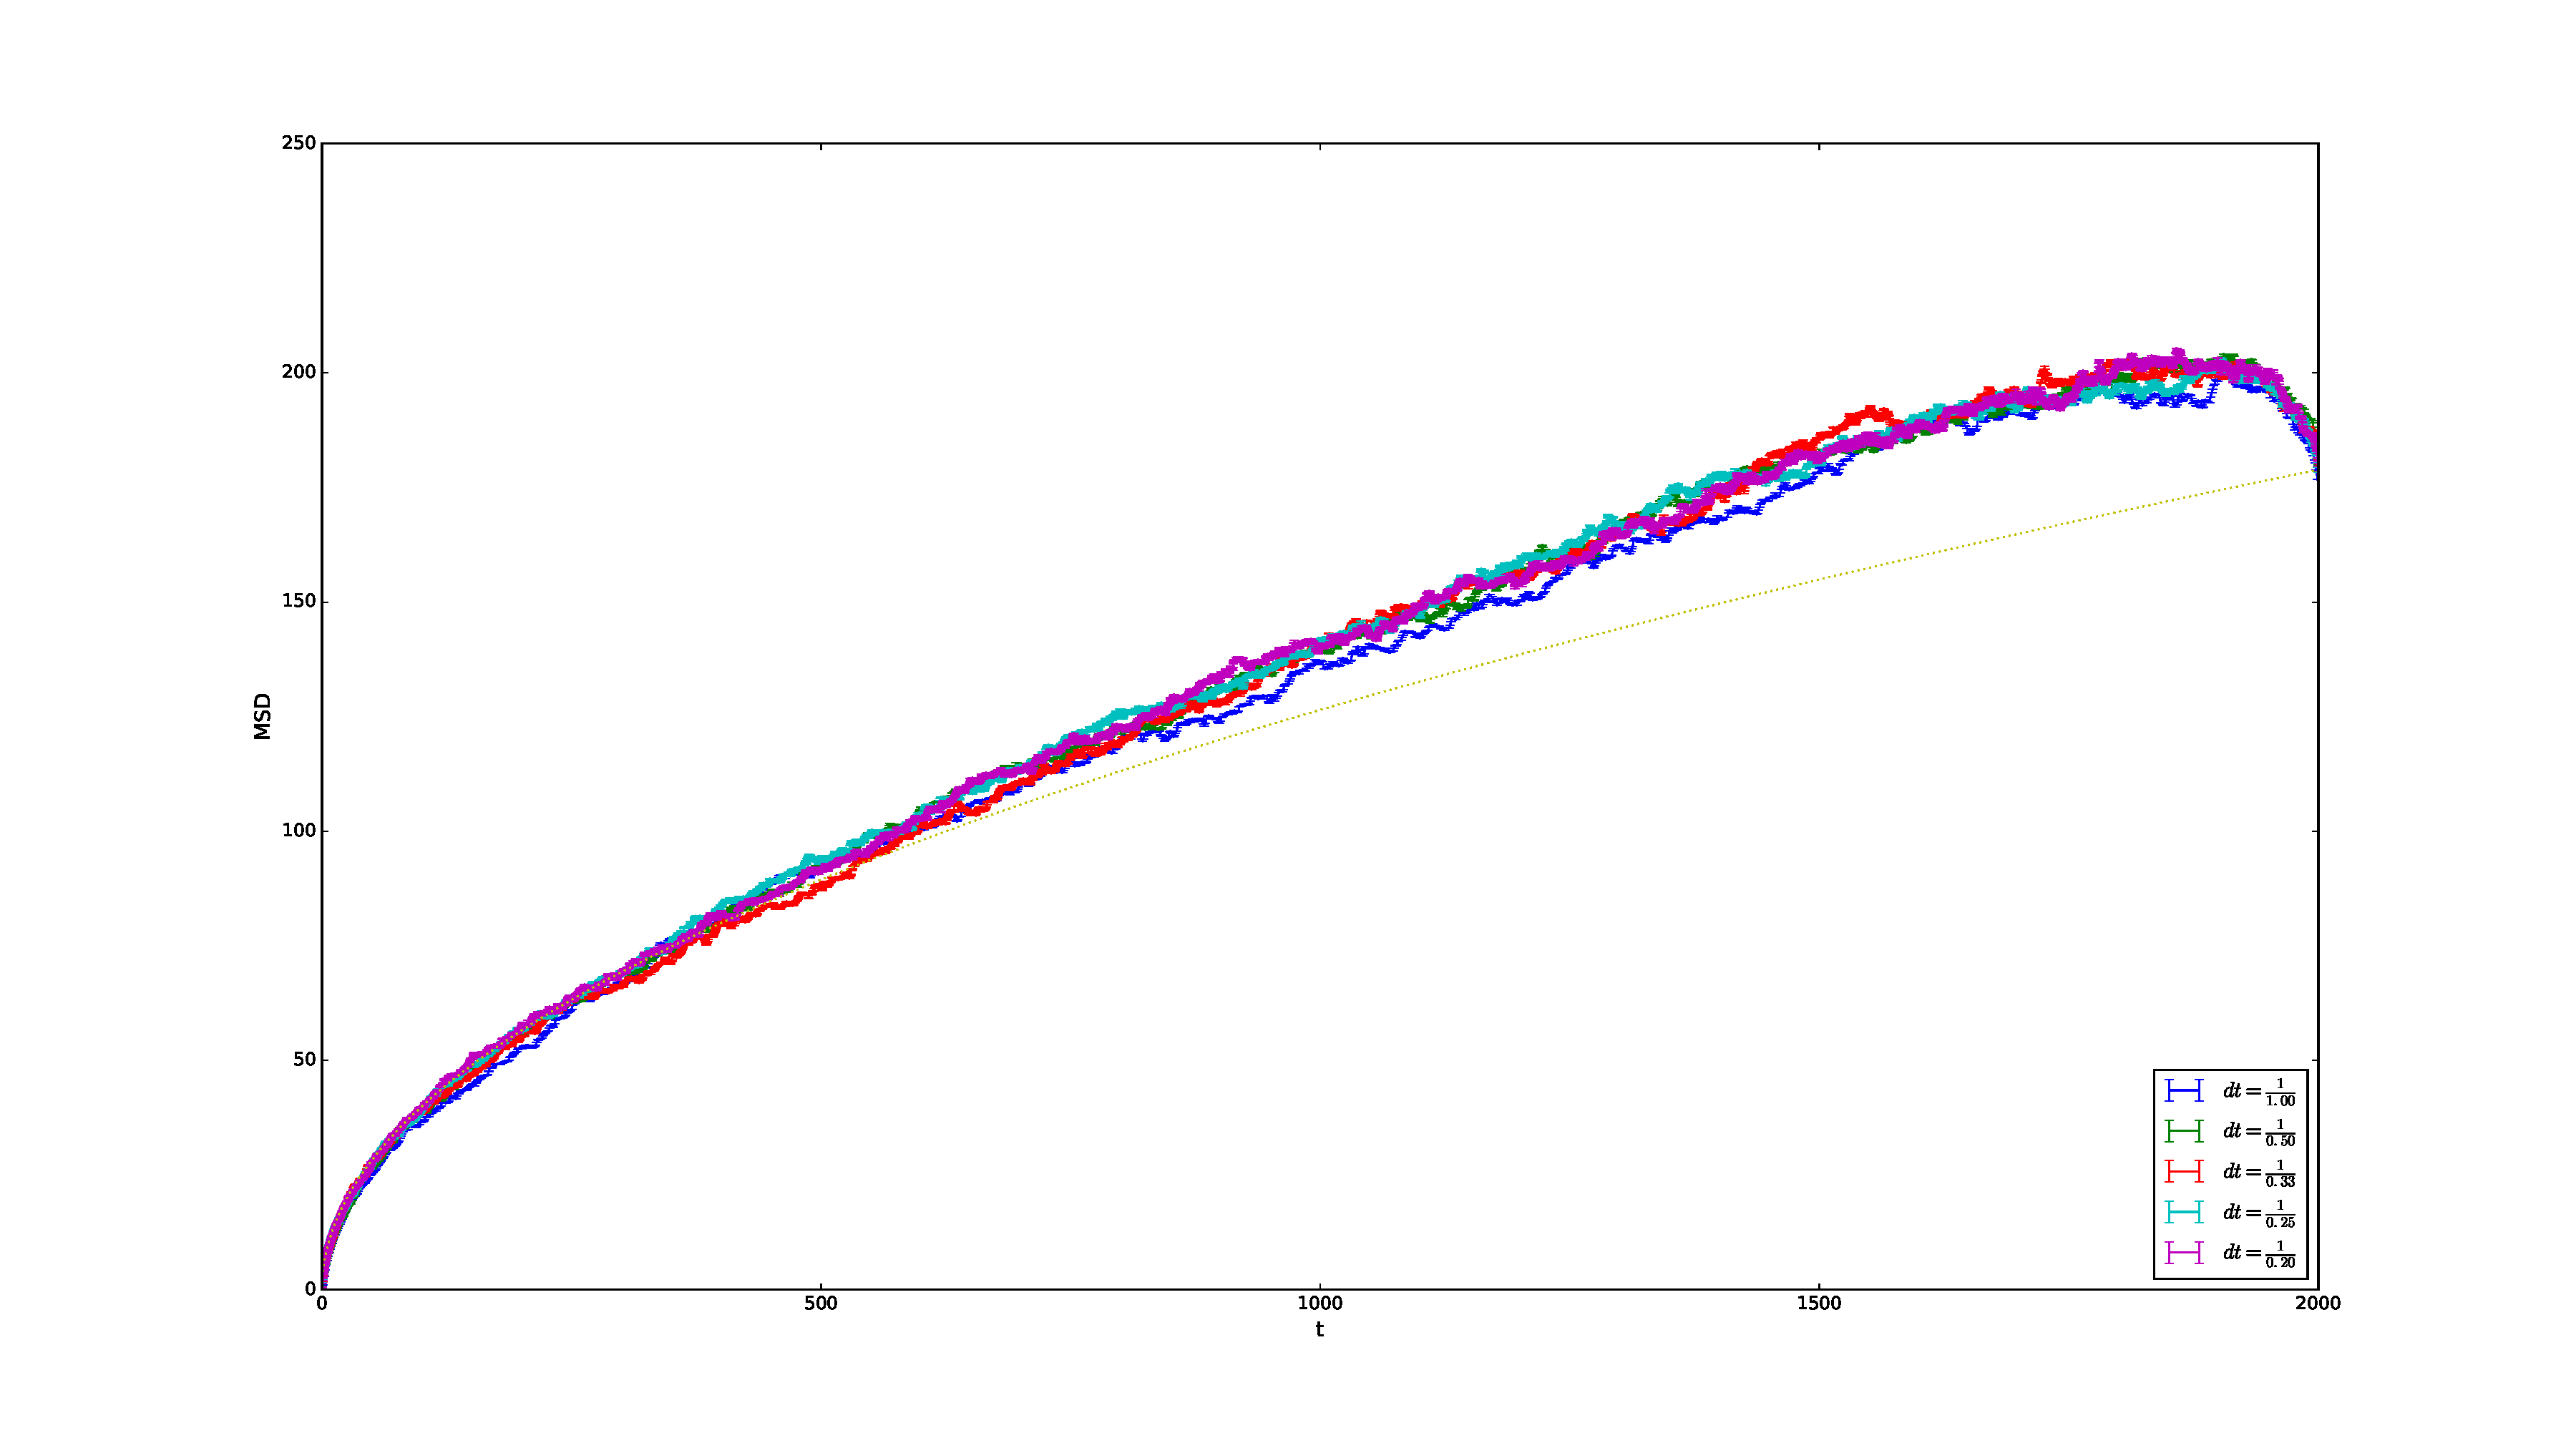
\includegraphics[width=\textwidth]{./dt_variert_bei_factor_1_lin.pdf}
\caption{variere dt bei gleichem Faktor 1}
% msd_ensemble_4000particles_log.pdf: 0x0 pixel, -2147483648dpi, 0.00x0.00 cm, bb=
 \centering
\end{figure}

\begin{figure}[h]
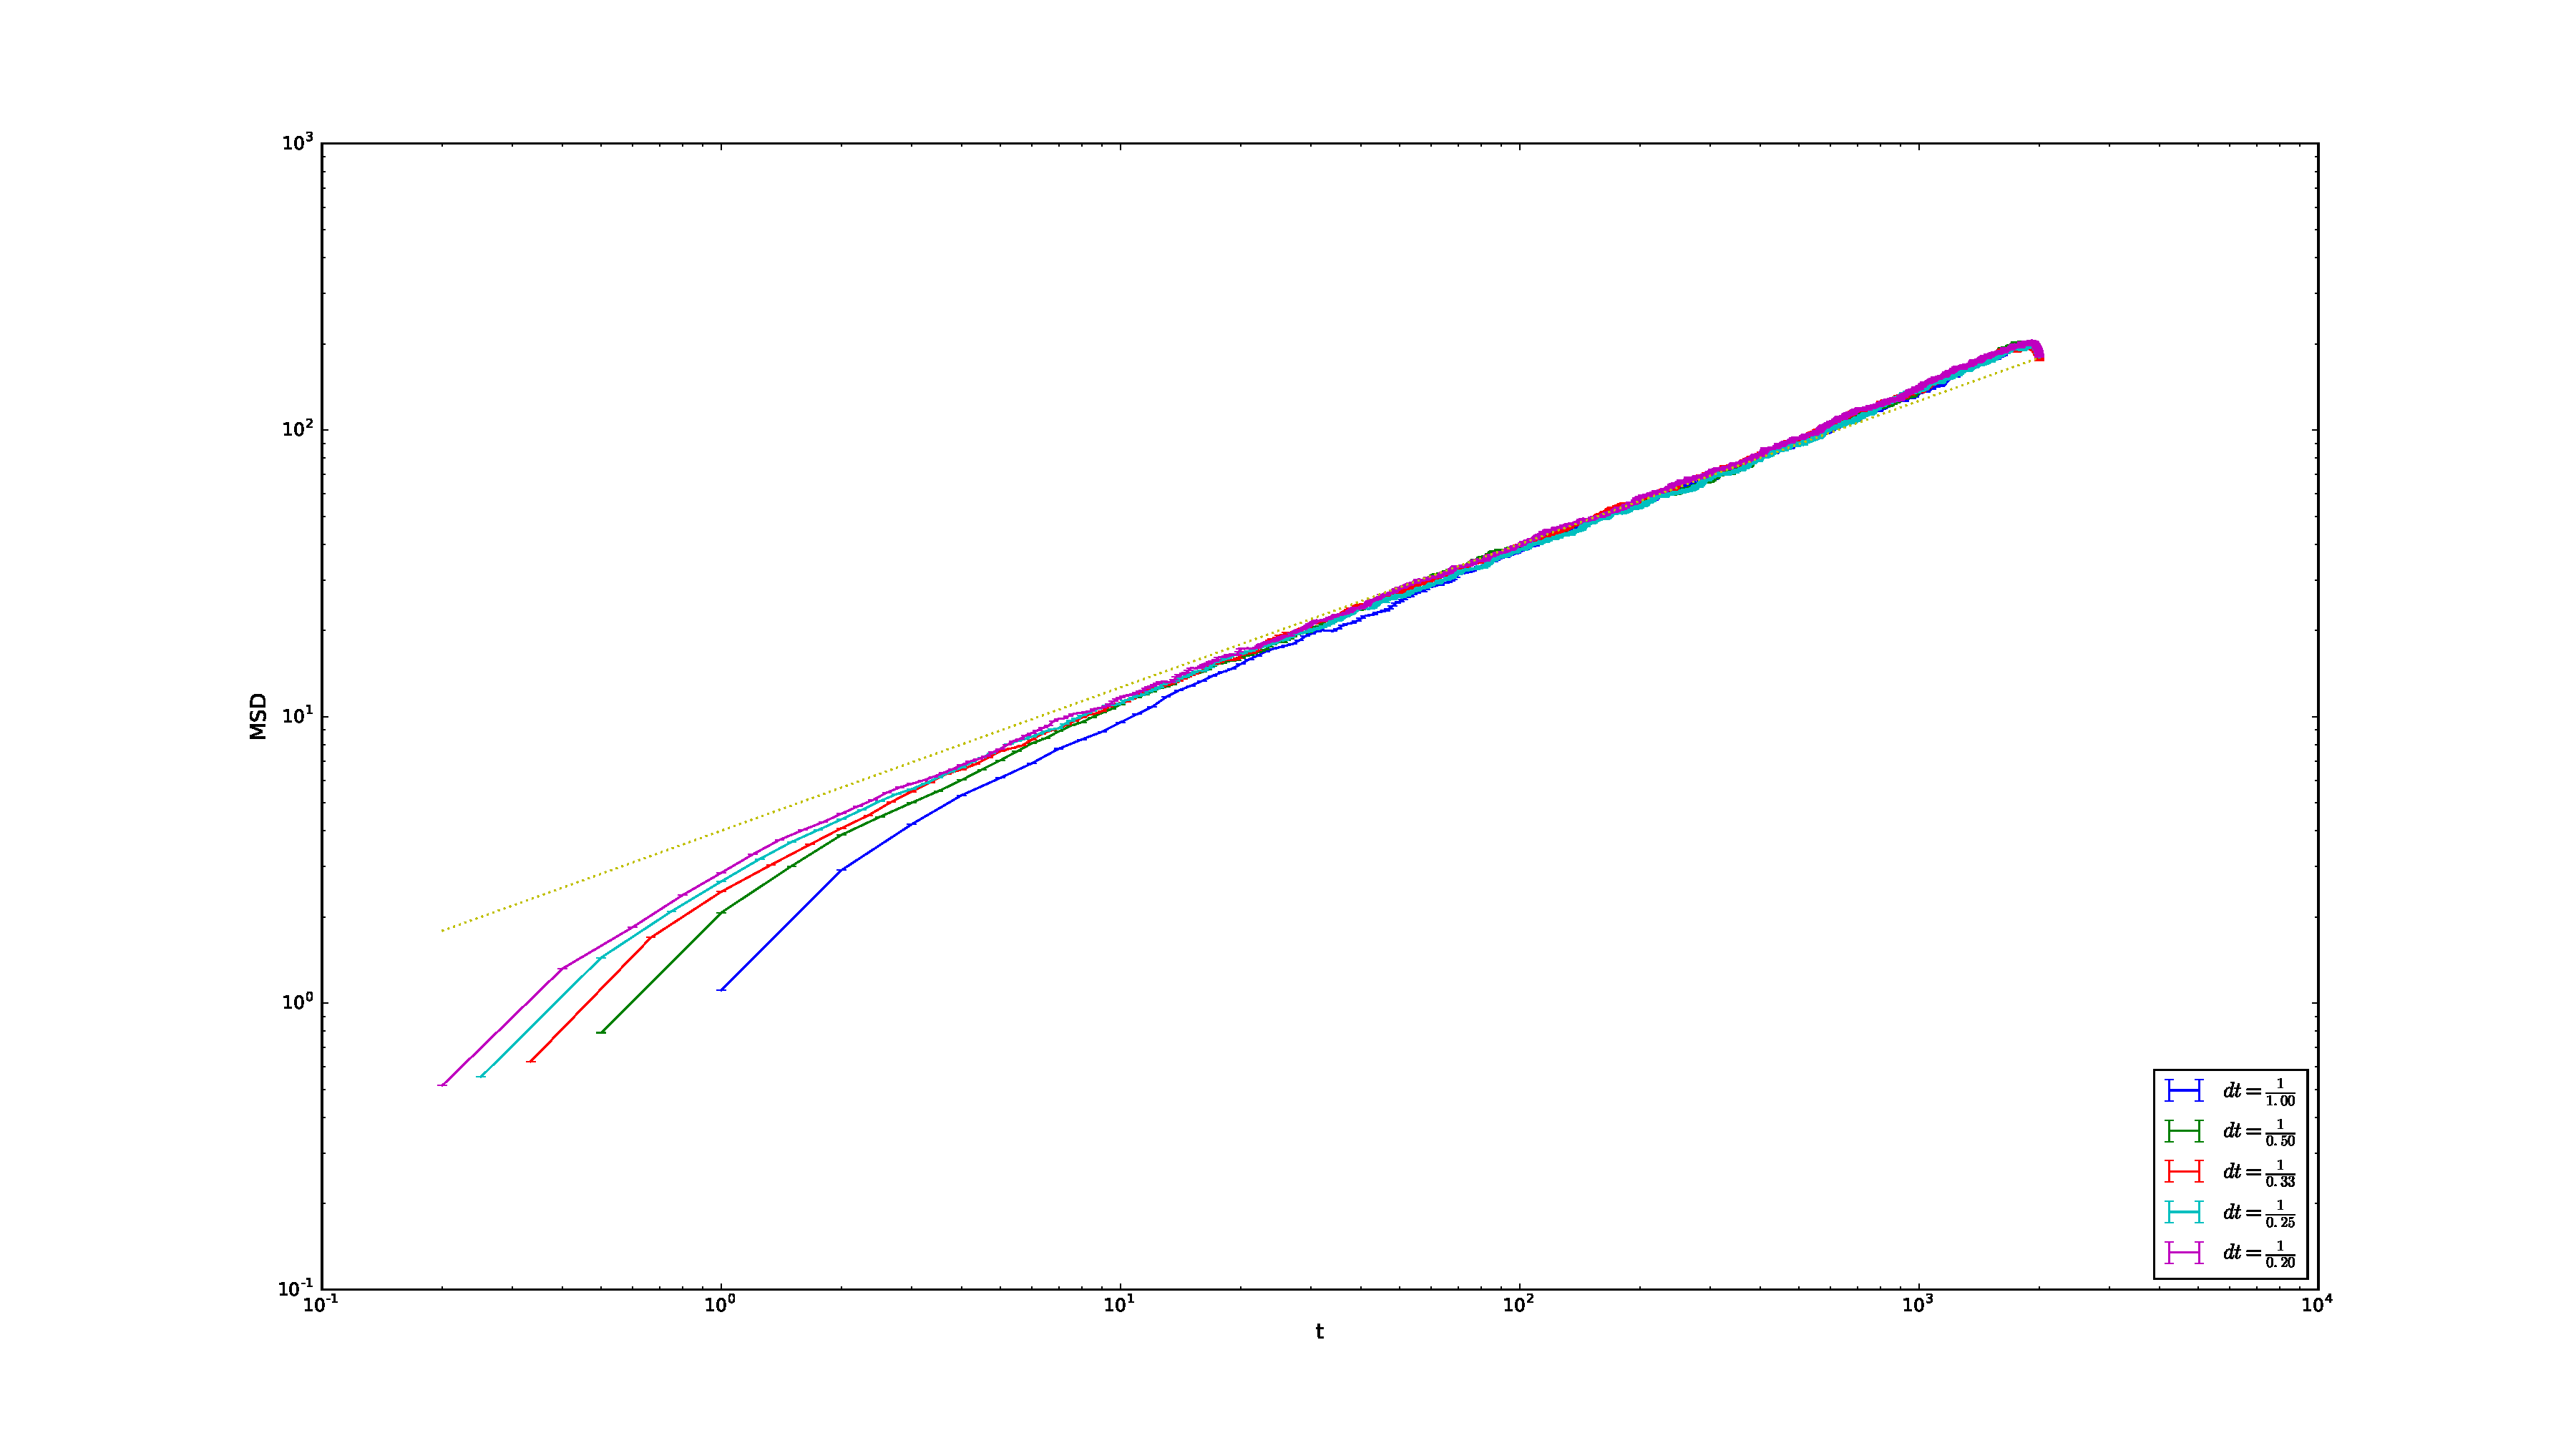
\includegraphics[width=\textwidth]{./dt_variert_bei_factor_1_log.pdf}
\caption{variere dt bei gleichem Faktor 1, logarithmisch}
% msd_ensemble_4000particles_log.pdf: 0x0 pixel, -2147483648dpi, 0.00x0.00 cm, bb=
 \centering
\end{figure}

\begin{figure}[h]
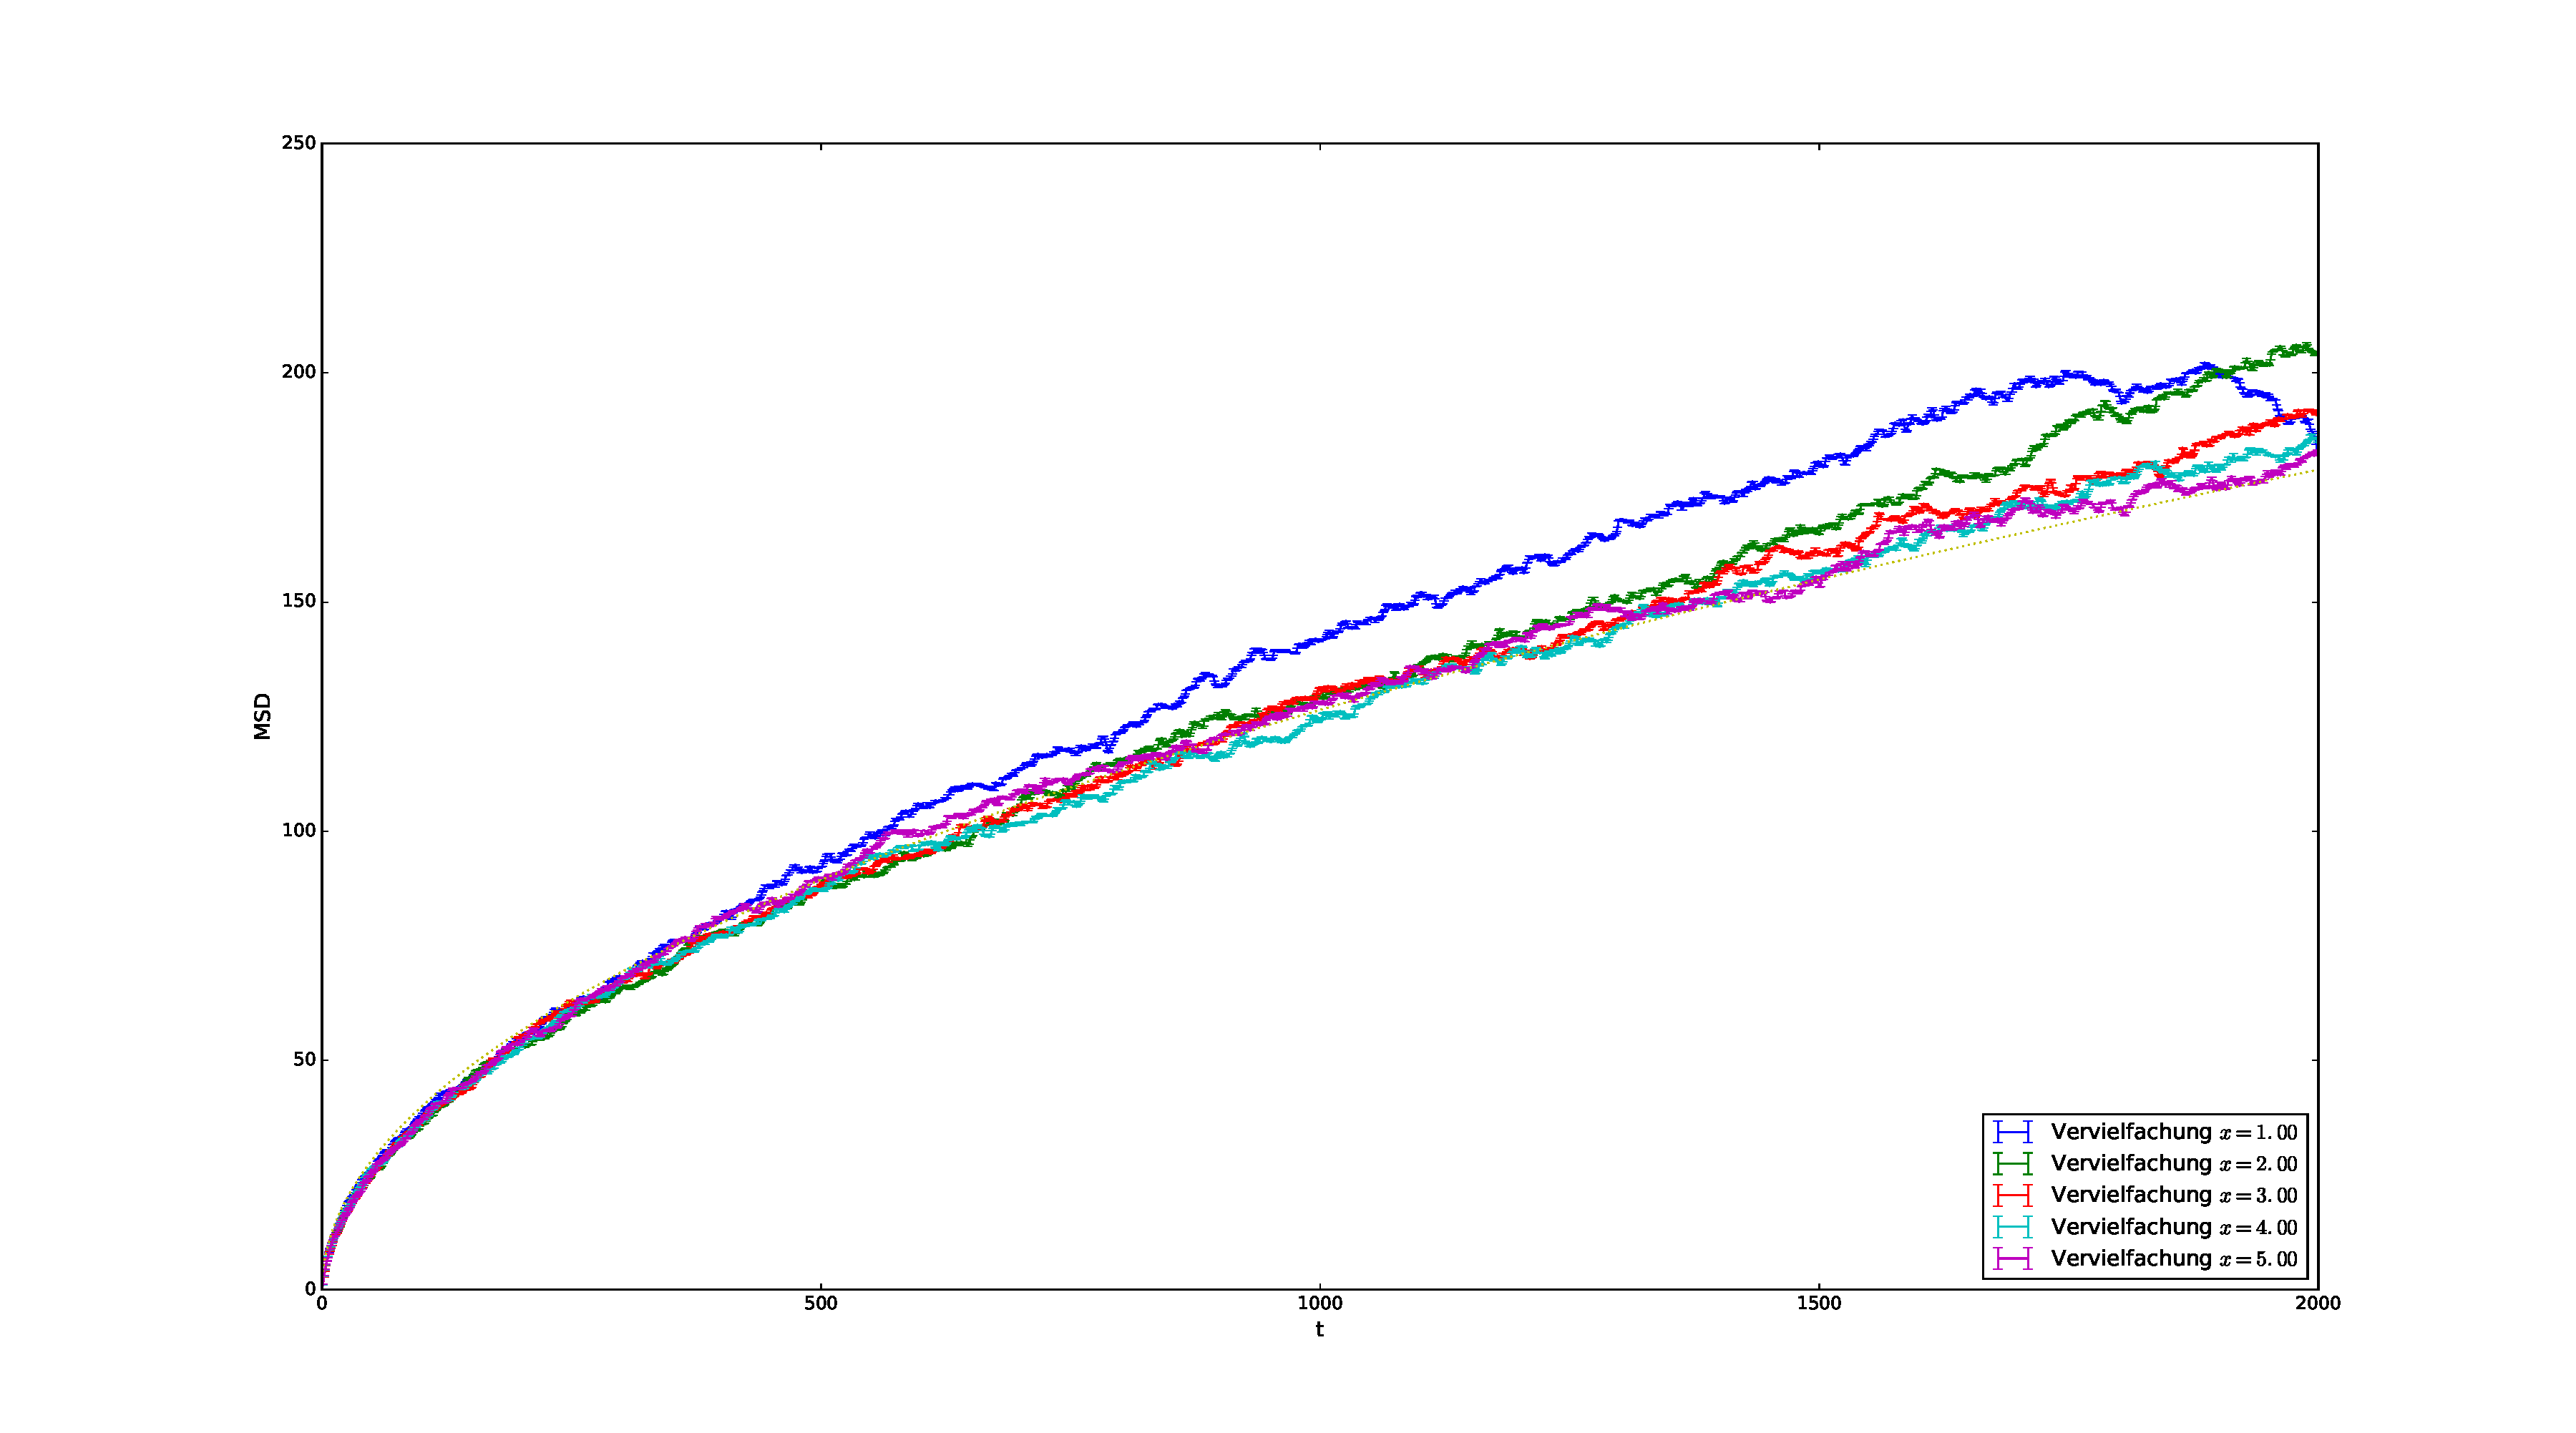
\includegraphics[width=\textwidth]{./faktor_variert_bei_dt_1_lin.pdf}
\caption{variere Faktor bei gleichem dt}
% msd_ensemble_4000particles_log.pdf: 0x0 pixel, -2147483648dpi, 0.00x0.00 cm, bb=
 \centering
\end{figure}

\begin{figure}[h]
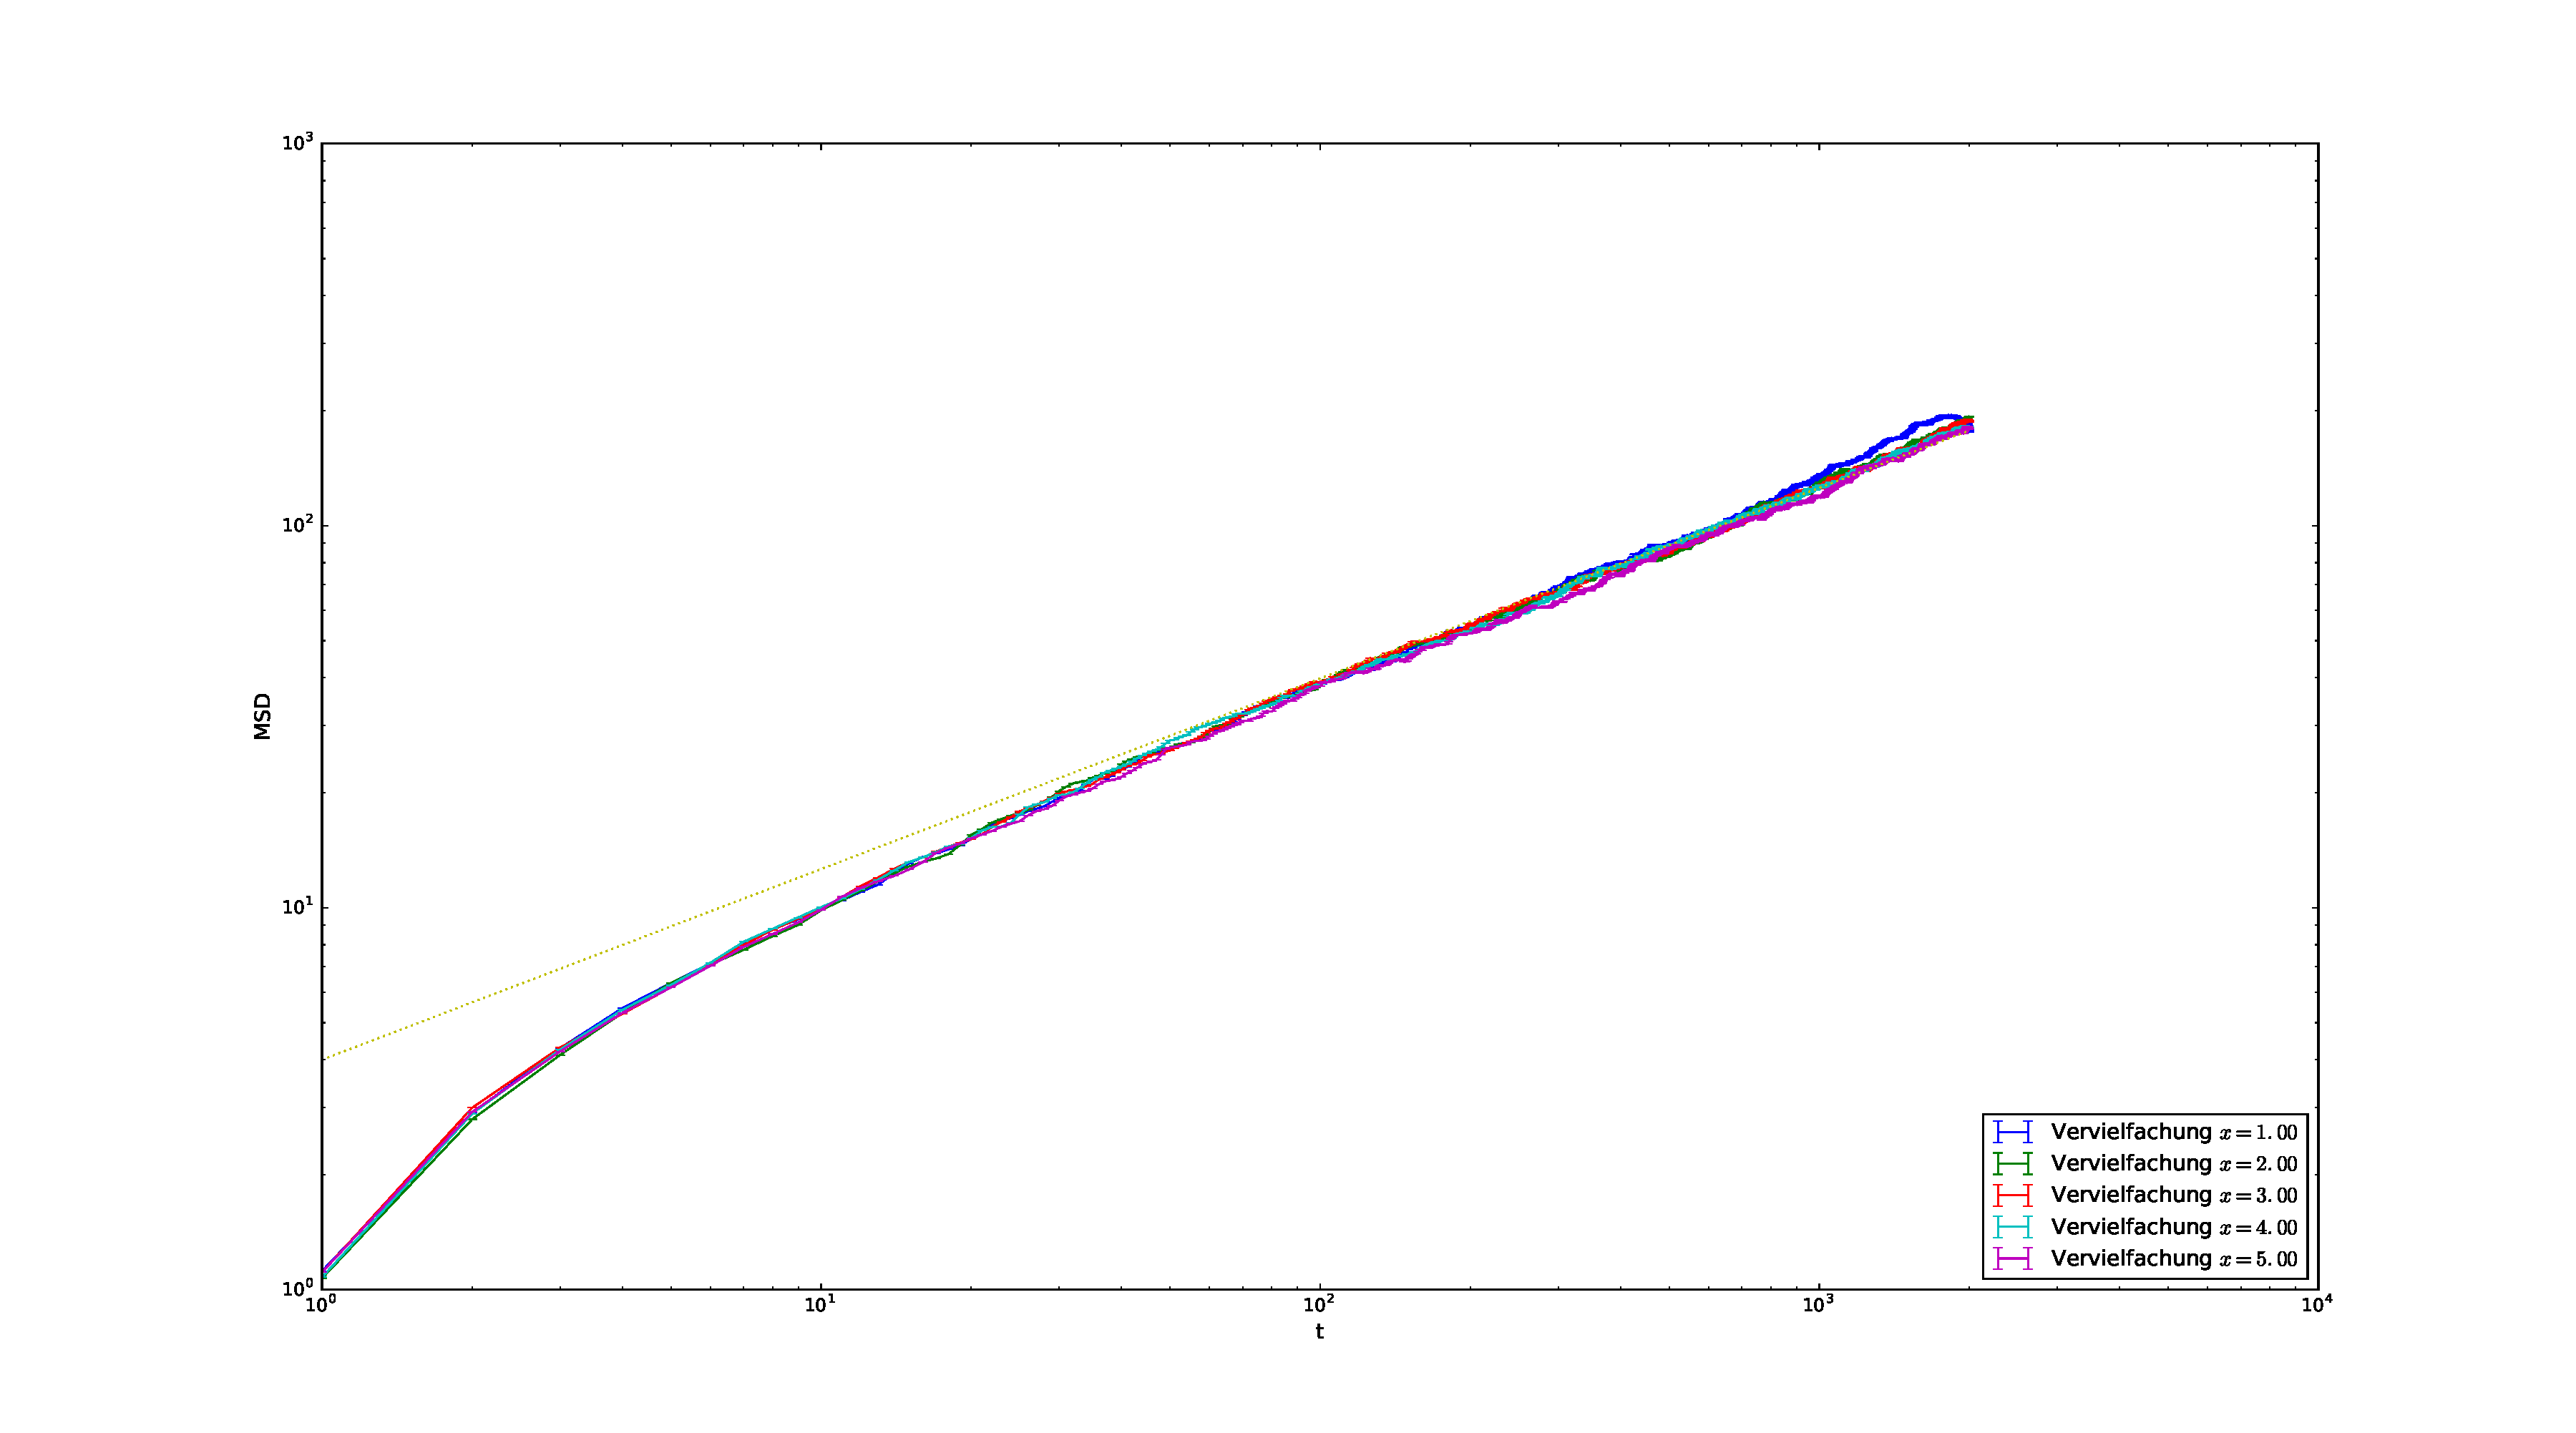
\includegraphics[width=\textwidth]{./faktor_variert_bei_dt_1_log.pdf}
\caption{variere Faktor bei gleichem dt, logarithmisch}
% msd_ensemble_4000particles_log.pdf: 0x0 pixel, -2147483648dpi, 0.00x0.00 cm, bb=
 \centering
\end{figure}

\chapter{Reaktions-Diffusions-Dynamics}
\chapter{Appendix}
\subsection{Code:Gebrochen-rationale Brownische Bewegung}
\lstinputlisting[language=Python]{../simulation.py}

\nocite{}

%\printindex
\bibliography{literatur}
\bibliographystyle{plain}

\end{document}